\chapter{Convergence diagnostics for Markov Chain Monte Carlo in Bayesian phylogenetics: the case of time-trees}

\epigraph{It is unbelievable that this stubborn darkness, this eternal eclipse, this flaw in geometry, this eternal cloud on virgin truth can be endured.}{Farkas (Wolfgang) Bolyai (1775-1856) talks about proving the parallel postulate in a letter to his son J\'anos Bolyai (1802-1860).}


%%%%%%%%%%%%%%%%%%%%%%%%%%%%%%%%%%%%%%%%%%%%%%%%%%%%%
%%%%%%%%%%%%%%%%%%%%%%%%%%%%%%%%%%%%%%%%%%%%%%%%%%%%%
\section{Motivation}
\label{sec:intro}

Markov chain Monte Carlo (MCMC) methods have become a standard tool for approximating complex posterior distributions encountered in Bayesian inference~\citep{Robert2011}.
In phylogenetics, most if not all Bayesian approaches rely on MCMC for approximating the posterior distribution of trees~\citep{Li2000,Suchard2001,Huelsenbeck2001b}.
These methods rely on constructing a Markov chain whose stationary distribution is the (target) distribution one wishes to sample from.
A fundamental issue is to determine when the chain has reached stationarity and samples are being drawn from the target distribution.
Whilst much attention has been given to this issue in the statistical literature, most diagnostic methods assume univariate, continuous parameter spaces.
Discrete, high-dimensional parameter spaces such as those encountered in phylogenetics pose additional challenges to development of effective convergence diagnostic tools.
In her review of the geometry of tree space, \cite{StJohn2017} argues that the power of the tree/phylogeny model ``comes from the property that adds the complexity: the vast number of trees to explain different possible evolutionary scenarios'' (pg e83).
As argued by~\cite{Drummond2015}, the complexity of phylogenetic space can be seen as a major reason for the development of specialised software for Bayesian phylogenetics as opposed to the use of common Markov Chain Monte Carlo (MCMC) packages such as Stan~\citep{Carpenter2017} and JAGS~\citep{Plummer2003}. 

Available methods for diagnosing convergence of MCMC for Bayesian phylogenetics include tracking clade (split) frequencies both within and between chains~\citep{Nylander2008}, multi-dimensional scaling of tree distance matrices~\citep{Hillis2005,Matsen2006} and network-based clustering~\citep{Whidden2015}. 
These methods are mostly graphical in nature, and only recently have more formal convergence metrics been proposed~\citep{Whidden2015,Lanfear2016}.
An important thing to notice is that it is not possible to say with complete certainty when a Markov chain has converged to its target distribution.
Rather, convergence tools are designed to identify failure to converge.
As argued by~\cite{Mossel2005}, when the data do not conform with the model (e.g., come from a mixture of trees rather than a single tree) apparent convergence can be misleading.
\cite{Cowles1996} and~\cite{Brooks1998} further reinforce the point that multiple convergence diagnostics need to be employed in order to mitigate the risk of determining convergence when in fact chains have not reached the desired target.
Thus, no single method or tool is likely to supersede all the others, as there are cases where one method fails to detect problems but others identify failure to converge. 
Successful application of convergence detection tools fundamentally depends on combining several metrics/tools in one coherent framework~(e.g. the approaches of~\cite{Nylander2008} and~\cite{Lanfear2016}).
An additional issue with currently available methods is that most assume either unrooted trees and/or contemporaneous sequences, limiting their applicability in cases where one deals with time-calibrated phylogenies (time-trees).
While~\cite{Warren2017} attempt to integrate most of the popular visualisation methods -- along with some quantitative indicators -- into one framework, their approach is infeasible for large time-calibrated phylogenies.

This chapter is a companion to Chapter 2, where I discuss transition kernels for Metropolis-Hastings MCMC and employ several of the methods described/developed here to assess convergence and performance.
My goal here is to expand upon the approach of~\cite{Warren2017} and make the necessary adaptations to accommodate time-calibrated trees with hundreds of taxa.
In what follows I review  some key concepts in Bayesian phylogenetics as well as the state-of-the-art for convergence diagnostics in MCMC applied to Bayesian phylogenetics.
I then proceed to discuss the limitations of available methods when dealing with time-calibrated trees and suggest adaptations.
My ultimate goal is to investigate a statistically useful representation of tree space and develop an analysis pipeline that can aid practitioners diagnose their MCMC runs when performing phylodynamic analyses for the increasingly larger data sets found in practice.

\subsection{Tree metrics}
\label{sec:metrics}

A key step in characterising phylogenetic space is constructing valid metrics on it.
A tree (phylogeny) metric is a mapping $d_\sigma : \boldsymbol \Psi \times \boldsymbol \Psi \to [0, \infty)$ that satisfies (i) $d_\sigma(u, v) \geq 0$; (ii) $d_\sigma(u, v) = 0 \iff u = v$;  (iii) $d_\sigma(u, v) = d_\sigma(v, u)$ and (iv) $d_\sigma(u, w) \leq d_\sigma(u, v) + d_\sigma(v, w)$ for any pair of trees $u, v$. 
For convenience, I let $\sigma$ be an indexing parameter so that we can distinguish between different metrics and study their properties.

A comprehensive review of available tree metrics would be out of the scope of this chapter.
Instead, I review a few important metrics that capture different aspects of phylogenetic space.
\cite{Robinson1981} propose a metric to compare unrooted tree topologies based on a tree operation $\alpha(u, v)$ that removes (contracts) all edges from $u$ that are not present in $v$, creating $u \wedge v$.
The reverse operation $\alpha^{-1}$ in turn adds edges to $u \wedge v$ to create $v$.
Let $n_\alpha$ and $n_{\alpha^{-1}}$ be the numbers of $\alpha$ and $\alpha^{-1}$ operations between $u$ and $v$.
Then the Robinson-Foulds (RF) metric is $d^{\text{RF}}(u, v) = n_\alpha + n_{\alpha^{-1}}$.
In other words the RF metric counts (twice) the number of internal branches/edges that differ between two phylogenies.
Another important tree metric is the so-called subtree prune-and-regraft (SPR)~\citep{Allen2001}.
Similarly to the above, let $\beta$ be an operation that picks an edge $e$ in $u$, prunes the subtree subtended by $e$ and regrafts this subtree at another edge $f$, creating a new tree $v$.
The SPR metric between $u$ and $v$ counts how many $\beta$ operations are necessary to turn $u$ into $v$. 
SPR is biologically interpretable and can also be used to construct useful representations of phylogenetic space (see Section~\ref{sec:graph}).
While there exist relatively efficient fixed parameter algorithms, computing the SPR metric is NP-hard.
As with the RF metric, SPR only captures differences in branching order (topology), not branch lengths.

To address this limitation,~\cite{Kuhner1994} proposed to calculate the square root of the sum of the squared differences of the internal branch lengths corresponding to shared bipartitions between $u$ and $v$.
While this adaptation does allow comparing branch lengths, it includes topological differences only implicitly.
As an advantage however is that there are very efficient, linear time algorithms available to compute the KF distance between pairs and lists of trees~\citep{Pattengale2007}.
In their excellent review of analytical results on tree metrics,~\cite{Steel1993} propose a simple and easy to compute metric that accounts for branch length differences, called the~\textit{path length} difference metric, henceforth called Steel-Penny (SP).
Let $d_{ij}^\tau$ be the sum of branch lengths separating tips $i$ and $j$ in phylogeny $\tau$. 
The SP metric computes the squared differences of path lengths by two trees $x$ and $y$ as $d_{\text{SP}}(x, y) = \sqrt{\sum_{1 \leq i \leq j \leq n} (d_{ij}^x - d_{ij}^y)^2 }$.

\cite{Kendall2016} proposed a new metric that can be thought of as a compromise in terms of applicability and computational complexity and that allows for the comparison of topology and branch lengths at the same time by cleverly encoding the phylogenies.
For a phylogeny $u$, define $m_{i,j} \in V_u$ to be the first node which is simultaneously the parent of $i$ and $j$,~\textit{i.e.}  $m_{i,j}$ is the most recent common ancestor (MRCA) of $i$ and $j$.
Then we are prepared to construct the vector with all $n(n-1)/2$ unique pairs of MRCAs, supplemented by $n$ entries with value $1$ at the end,  $\boldsymbol m(u) = \left( m_{1,2}, m_{1, 3}, \ldots, 1, 1, \{ n\:\text{times}  \}, 1 \right)$.
Let $W_{i,j}$ be the branch length associated with $m_{i,j}$ and define $l_i$ to be the root-to-tip path length for tip $i$ in $u$.
Then we can define\footnote{Hence $|\boldsymbol m(u)| = |\boldsymbol W(u)| = n(n+1)/2$.} $\boldsymbol W(u) = \left( W_{1,2}, W_{1,3}, \ldots, l_1, \ldots, l_n \right)$.
For $ 0 \leq \lambda  \leq 1$ we can combine topology and branch length and encode the phylogeny $u$~\textit{via} the vector $\boldsymbol\eta_\lambda(u) = (1-\lambda)\boldsymbol m(u) + \lambda \boldsymbol W(u)$.
Finally, we are prepared to define the Kendall-Colijn (KC) metric between two phylogenies $u$ and $v$ as $d_\lambda^{\text{KC}}(u, v) = ||\boldsymbol\eta_\lambda(u) -\boldsymbol\eta_\lambda(v)||$, where $||\cdot||$ is the the Euclidean or $L^2$ norm.
This metric combines topology and branch lengths, is continuous for any $\lambda \in [0, 1]$ and is straightforward to compute, specially when compared with the BHV and SPR metrics.

Finally, I describe two other metrics specifically designed for time-calibrated trees.
The first, which I shall call the clade-difference (CD) metric, takes two phylogenies $\tau_A$ and $\tau_B$ and asks how many different clades there exist between them and how different their heights are.
More formally, let $\boldsymbol C(x)$ be the set of clades of phylogeny $x$.
Then the CD metric can be defined as follows: for each clade $c_i \in \boldsymbol C(\tau_A)$, compute the height of the MRCA between the constituents of $c_i$ in $\boldsymbol C(\tau_B)$, $m_i$ and the corresponding clade in $\tau_A$.
Repeating the same procedure for $\tau_B$ we can then compute:
$$ d_{\text{CD}} (\tau_A, \tau_B) = \sqrt{  \sum_i\left[ \left(h(c_i) - h(m_i) \right)^2 \right]  + \sum_j \left[ \left(h(c_j) - h(m_j)\right)^2 \right].  } $$
The idea behind CD is to quantify big topological differences such that  if a clade moves  across the tree, the metric will penalise both the difference between the height of that node and the root in $\tau_A$ and back down to the height of the corresponding node in $\tau_B$.
The second metric is the rooted branch score (BS) proposed by~\cite{Heled2010} which computes the Euclidean distance in branch lengths between shared clades.
Let $b(\tau, c)$ be the length of the branch subtending $c$ in $\tau$ if $c \in \boldsymbol C(\tau)$ and $0$ otherwise.
Then we are prepared to define
$$d_{\text{BS}}(\tau_A, \tau_B) = \sqrt{ \sum_{c \in \boldsymbol C(\tau_A) \cup \boldsymbol C(\tau_B) } \left( b(\tau_A, c) - b(\tau_B, c) \right)^2 }  .$$
Fortunately, efficient implementations do exist for these metrics, e.g. in the JEBL library (\url{https://github.com/rambaut/jebl2}).

\section{Convergence of Markov chain Monte Carlo methods} % Related work
\label{sec:litrev}

I now move on to review the existing literature on quantifying and visualising MCMC convergence for Bayesian phylogenetics.
My main goal is to explore how several approaches capture different aspects of the process under analysis and discuss their shortcomings when dealing with the types of phylogenies I am interested in this thesis: time-calibrated phylogenies, with large numbers of taxa and complex tip sampling structures.
Before I proceed, however, it is important to make clear that one can never positively assert the convergence of a finite Markov chain to a stationary distribution.
In contrast, convergence detection/assessment is done in a negative fashion: one~\textit{fails to detect lack of convergence} and hence asserts that~\textbf{the chain appears to have converged}.
Another important remark is that~\textbf{convergence is a global feature},~\textit{i.e.} for high-dimensional models with many parameters, one can only assert that the run appears to have converged if that is true of \textit{all} parameters.

\subsection{Convergence diagnostics for continuous parameters}
\label{sec:continuous}

In Bayesian phylogenetics, sometimes researchers are interested in gathering inference about what I will hereafter call ``continuous parameters''\footnote{Called ``scalar estimands'' elsewhere~\citep{Gelman2014b}. Here, however, I am also interested in vector-valued quantities, such as root probabilities, population sizes,  etc.}.
These include evolutionary and migration rates, Markov evolutionary model parameters (e.g. $\kappa$ in the HKY model), amongst many others.
Fortunately, this kind of parameter is the standard in models used in the statistical literature at large, which means there is a large body of work on how to detect convergence for continuously-defined quantities in MCMC (see~\cite{Cowles1996} and~\cite{Mengersen1999} for reviews).

Let $\boldsymbol\theta = \{\theta^{(1)}, \theta^{(2)}, \ldots, \theta^{(M)}\}$ be a collection of $M$ samples from a single run of MCMC.
Since from a Bayesian perspective all computations should be done from the target posterior $p$ (see Chapter 1), we need to make sure that $\boldsymbol\theta$ is a sample from that distribution.
The first thing to notice is that the samples in $\boldsymbol\theta$ are~\textit{correlated} and hence do not constitute a proper sample from the target.
Hence we need to quantify the amount of~\textit{autocorrelation} between the samples, which in turn will give us an estimate of the~\textit{effective} number of samples from $\pi$ contained in $\boldsymbol\theta$, \textit{i.e.} for any $n \leq M$ we want to assess the dependence between $\theta^{(n)}$ and $\theta^{(n + 1)}$.
I will now make these statements precise, following the notation of~\cite{Geyer2011} as much as possible, occasionally borrowing from the Stan manual~\citep{StanTeam2017} as well.

It is often the case with MCMC that we are interested in quantity $Y = g(\theta)$, where $g(\cdot)$ a real-valued function, but the distribution of $Y$ cannot be derived analytically and hence expectations of the form $\mu = E[g(X)]$ cannot be computed exactly. 
An estimate of $\mu$ can be obtained from $\boldsymbol\theta$ as:
\[ \hat{\mu}_M = M^{-1}\sum_{i = 1}^M g(\theta^{(i)}). \]
If the samples in $\boldsymbol\theta$ were independent, we could say that $\hat{\mu}_M \approx \text{Normal} (\mu, \sigma^2/M)$ using the central limit theorem (CLT).
However, because by construction the samples are correlated, we need to take that into account when estimating the variance of $\hat{\mu}_M$.
Let $\gamma_k = \text{cov}(g(\theta^{(i)}), g(\theta^{(i + k)}))$ be the autocovariances and write the variance $\sigma^2$ as 
\[ \sigma^2 =  \gamma_0 + 2\sum_{k=1}^\infty \gamma_k,\]
and the autocovariances can in turn be estimated as 
\begin{equation}
\label{eq:autocovs}
 \hat{\gamma}_k = M^{-1}\sum_{i = 1}^{M-k}[g(\theta^{(i)}) - \hat{\mu}_M][g(\theta^{(i + k )}) - \hat{\mu}_M]
\end{equation}

With a estimate $\hat{\sigma}_M$ of the variance we can then define the \textbf{effective sample size (ESS)}:
\begin{align}
 \label{eq:ESSa}
 n_{\text{eff}} &= M\frac{\sigma^2}{\hat{\sigma}_M}, \\
  \label{eq:ESSb}
 &= \frac{M}{ 1 + 2\gamma_0^{-1}\sum_{k = 1}^\infty \gamma_k},
\end{align}
which captures the number of samples in the MCMC sample $\boldsymbol\theta$ that are effectively independent and hence can be used for inference\footnote{In practice the upper limit of the summation in the denominator of Eq (\ref{eq:ESSb}) is substituted by a finite bound $K$. See~\cite{Geyer2011} and references therein for details on the determination of $K$ and the estimation of $n_{\text{eff}}$.}.
In Bayesian phylogenetics practice, ESS is at the core of most convergence assessment -- for continuous parameters --, the common recommendation being that all parameters in a MCMC run have $n_{\text{eff}} > 200$.
The rationale for this recommendation seems to be that the variability in most quantities of interest is such that a sample size of $200$ should allow for precise computation of most functionals.
In this chapter I will use the \verb|effectiveSize()| in the~\textbf{coda} package~\citep{Plummer2006} and the routines in the package Tracer v1.7~\citep{Rambaut2018} to compute ESSs.
Note however that while the ESS is a useful tool for assessing mixing, it is designed to deal with one chain (run) at a time.

With respect to~\textit{convergence} to the target distribution, however, ESS may be misleading in the sense  that chain stuck in a mode can have high ESS but has not converged to the target distribution because it has not adequately explored all of the modes proportional to their probability.
A powerful technique for assessing convergence is to run several parallel chains from overdispersed starting points and determine whether they converge to the same distribution.
Suppose $K$ runs of $M$ iterations each are available, \textit{i.e.}, we have $\boldsymbol\theta_i, i = 1, 2, \ldots K$.
The between sample variance can be written as
\begin{equation}
\label{eq:Between}
 B = \frac{M}{K-1} \sum_{k = 1}^K \left(\bar{\theta}_k - \bar{\bar{\theta}}\right)^2, 
\end{equation}
where $\bar{\theta}_k = M^{-1}\sum_{i = 1}^M\theta_k^{(i)}$ and $\bar{\bar{\theta}} = K^{-1}\sum_{k=1}^K\bar{\theta}_k$.
Now we can define the within variance as 
\begin{align}
\label{eq:Within}
 W &=  K^{-1}\sum_{k = 1}^K s_k^2,\\
 s_k^2 & = (M-1)^{-1} \sum_{i = 1}^M \left(\theta_k^{(i)} - \bar{\theta}_k\right)^2.
\end{align}
Finally we can define the~\textbf{potential scale reduction factor} (PSRF)~\citep{Gelman1992}:
\begin{equation}
 \label{eq:PRSF}
 \hat{R} = \sqrt{\frac{ (M-1)W +  B }{MW}}.
\end{equation}
At convergence, $\hat{R} < 1.1$, providing a univariate measure of convergence across chains (for a given parameter).

Finally, I note  that we are usually interested in complex models, where correlation between parameters is frequently a feature of the posterior.
I detail the approach of~\cite{Vats2015} that attempts to provide an overall measure of convergence by means of a~\textbf{multivariate effective sample size (mESS)}.
The idea is to accommodate posterior dependence between parameters by jointly considering all parameters at once and estimating their variance-covariance matrix.
For $M$ samples, the mESS is defined as :
\begin{equation}
 \label{eq:multiESS}
 n_{\text{eff}}^m = M\left(\frac{\text{det}(\boldsymbol\Lambda)}{\text{det}(\boldsymbol\Sigma)}\right)^{1/p},
\end{equation}
where $p$ is the number of parameters under analysis and $\text{det}(\boldsymbol\Lambda)$ and $\text{det}(\boldsymbol\Sigma)$ are the determinants of the sample covariance matrix and the Monte Carlo covariance matrix, respectively.
Notice that similarly to the ESS, when samples are independent, $\boldsymbol\Lambda = \boldsymbol\Sigma$ and hence $ n_{\text{eff}}^m = M$.
Routines to compute the mESS are implemented in the R package~\textbf{mcmcse}~\citep{Flegal2017}.

These procedures can also be used to determine the lower bound on the multivariate ESS to achieve a certain level of confidence.
If $\epsilon$ is the fraction of the variance due to Monte Carlo error and we would like to collect enough samples to have $(1-\alpha)\times 100 \%$ confidence, the bound becomes
\begin{equation}
 \label{eq:mESSbound}
  n_{\text{eff}}^m  \geq \frac{\pi2^{2/p}}{(p \Gamma(p/2))^{2/p}} \frac{\chi^2_{1-\alpha, p}}{\epsilon^2},
\end{equation}
where $\Gamma(\cdot)$ is the (analytically continued) Gamma function and  $\chi^2_{1-\alpha, p}$ is the appropriate quantile of a chi-squared distribution with $p$ degrees of freedom.
For instance, if $p=1$ and one would like for the Monte Carlo error to be no more than $5\%$ ($\epsilon = 0.05$) of the total variance and would like to have $95\%$ confidence, we would need an ESS of at least $6146$.
If Monte Carlo error is allowed to be $10\%$ ($\epsilon = 0.10$) the minimum required ESS decreases to $1516$, a figure more than seven times higher than the folkloric recommendation for $\text{ESS} \geq 200$ in phylogenetics\footnote{See for instance~\url{http://beast.community/analysing_beast_output}.}.
If one adopts this recommendation --\textit{i.e.} fixes ESS = 200 --, keeping $\alpha = 0.05$ gives $\bar{\epsilon} = 0.27$, meaning this recommendation leads to inferences being drawn from samples where nearly 30\% of the variance is due to Monte Carlo error.

\subsection{Convergence in phylogenetic space}
\label{sec:treespaceconv}

I now move on to present the state of the art for convergence metrics specifically designed for phylogenetics.
Their limitations are also explicitly discussed.

\subsection{Clade frequencies}
\label{sec:awty}

When diagnosing MCMC convergence in phylogenetic space, simply inspecting the traces for, say, the phylogenetic likelihood, might be misleading because two phylogenies with similar likelihoods may not be necessarily close in phylogenetic space.
The approach of~\cite{Nylander2008} is to analyse clade/split frequencies to this end.
The program AWTY (short for ``are we there yet?'') developed by~\cite{Nylander2008} provides graphical facilities for assessing convergence by analysing various aspects of the distribution of sampled clades.
I shall describe and discuss these features now.

For $ i = 1, 2, \ldots, |\boldsymbol C|$, let $\boldsymbol X_i = \{X^{(1)}, X^{(2)}, \ldots, X^{(M)}\} \in [0, 1]^M$ be a collection of samples from a Markov chain such that $X^{(j)}_i = 1$ if clade $i$ was sampled in the $j$-th iteration and $0$ otherwise.
Also, for $s_i = \sum_k X_i^{(k)}$ we call $f_i = s_i/M$ the \textit{frequency} of clade $i$.
By plotting clade frequencies estimated in two independent runs against each other (scatterplot), one can assess whether both chains have converged to similar distributions.
Lack of convergence can be detected when points fall away from the identity ($x = y$) line.
For a single run, one useful diagnostic is plotting cumulative clade frequencies along the chain.
If these trajectories present long-term trends\footnote{I am not familiar with the original implementation of AWTY, but this could be made precise by for instance applying LOESS-based trend detection methods to the trajectories.}, it means clade frequencies have not stabilised, indicating lack of convergence.

When multiple (say $K$) runs are available, a very common univariate summary associated with clade frequencies is the \textbf{average standard deviation of split frequencies  (ASDSF)}:
\begin{equation}
 \label{eq:ASDSF}
%  C^{-1}\sum_{i = 1}^{C} \sqrt{(K-1)^{-1}\sum_{k=1}^K\left(f_{ik} - K^{-1}\sum_{k = 1}^K f_{ik}\right)^2}
 \delta_C = (K-1)^{-1/2}\sum_{i = 1}^{C}\sqrt{\sum_{k=1}^K\left(f_{ik} - K^{-1}\sum_{k = 1}^K f_{ik}\right)^2}
\end{equation}
where $C$ is the number of clades seen in all runs.
ASDSF is employed for instance in the software \verb|Mr Bayes|~\citep{Huelsenbeck2001a}, where an ASDSF of less than $0.01$ is taken as sign of convergence -- and used as a stopping rule.

Absence-presence plots show whether a particular clade was absent or present in the tree sampled at each iteration of the chain.
If there are long periods where the clade is either absent or present, this indicates the chain has not mixed well and might not have converged.
On the other hand, a trace plot of this kind where the indicator variable frequently switches between $0$ and $1$ indicates good mixing.
This notion of ``clade-switching'' can be made more precise (see section~\ref{sec:cladeSwitch}).
It should be noted however that tracking all clades present in a given run becomes exponentially more cumbersome as the number of taxa increases, quickly overwhelming any graphical diagnostic capabilities.

Finally, one can also plot the (phylogenetic) distance within and between runs using any of the metrics described above.
The idea is, again, that at convergence these sets of distances should be similar, and I discuss below (Section~\ref{sec:treeESS}) how to make this notion mathematically precise following~\cite{Whidden2015}.
In short, AWTY provides the following diagnostics: (i) scatterplot of clade frequencies; (ii) plot of cumulative  clade frequencies; (iii) absence-presence plots for clades and (iv) tree distances between and within runs.
See Figure 1 in~\cite{Nylander2008} for a graphical summary.
A modern incarnation of AWTY, RWTY~\citep{Warren2017} seeks to provide modern plotting routines to implement the AWTY framework in the R language.
RWTY also integrates other techniques not available from AWTY like multi-dimensional scaling visualisation (see below).
The implementation of RWTY is amenable to automation, insofar as it allows easy scripting and report generation using capabilities available for R.

\textbf{Limitations}

Most methods in AWTY (and RWTY) are visual, and hence do not provide precise quantitative measures to guide researchers toward a decision.
This in turn also means that these procedures are hard to automate, what hinders their application in automatic phylogenetic pipelines such as \verb|NextStrain|~\citep{Hadfield2017}.
As an example, consider the clade frequency scatter plots described above: what is an acceptable bound on the deviations in clade frequencies between two independent runs?
This question could be tackled with theoretical considerations and/or a careful empirical study, but neither~\cite{Nylander2008} nor~\cite{Warren2017} offer any insight into the matter.

\subsection{Clade switching}
\label{sec:cladeSwitch}

Here I describe  what to the best of my knowledge is a new metric for quantifying mixing in clade space.
Let $\boldsymbol X_i = \{X^{(1)}, X^{(2)}, \ldots, X^{(n)}\} \in [0, 1]^n$ be a collection of samples from a Markov chain such that $X^{(j)}_i = 1$ if clade $i$ was sampled in the $j$-th iteration and $0$ otherwise.
Also, for $s_i = \sum_k X_i^{(k)}$ we call $f_i = s_i/n$ the \textit{frequency} of clade $i$.
For $m_i = \min(n - s_i, s_i)$, it can be shown that the maximum number of transitions that can be observed from $\boldsymbol X_i$ is either $J_i = 2 m_i$
\footnote{Technically, $J_i$ depends on the first state $X_i^{(1)}$.
Suppose w.l.o.g. that $m_i = s_i$.
Then $J_i = 2 m_i - 1$ if $X_i^{(1)} = 1$ and $J_i = 2 m_i$ otherwise.
}.

When the chain is mixing well,~\textit{i.e.}, efficiently traversing phylogenetic space, we expect the indicators to be flipping between $0$ and $1$ as frequently as possible,  the maximum frequency depending on $f_i$.
Let $\delta_i = \Delta(\boldsymbol X_i)$, where $\Delta(\cdot)$ a function that counts the number of state transitions in $\boldsymbol X_i$.
Then $\sigma_i = \delta_i/J_i \in [0, 1]$ is a score that measures the relative efficiency of sampling by comparing how how many transitions happened compared to the theoretical maximum. 
This metric is quite similar to the Split Swap Rate of~\cite{Hoehna2008b}.

If the data are very informative, it is possible that some clade will have very high or very low posterior probabilities, meaning their indicators might never change.
These clades are not interesting for assessing mixing and I therefore restrict attention to clades with $0.4 \leq f_i \leq 0.8$.
This choice of ``interesting clades'' is tailored towards single chains.
When multiple chains are available,~\cite{Warren2017} propose tracking clades that have the highest changes in frequency across chains as these are more likely to be problematic.
A multi-chain version of the switching score could be devised to complement this latter approach by measuring mixing in addition to diagnosing convergence issues.

It should be noted that under mild regularity conditions, the techniques described in Section~\ref{sec:continuous} of Chapter 3 can be applied to binary variable such as the clade frequencies, hence the importance of the clade-switching approach is unclear.
One could, for instance, compute the univariate ESS for each clade of interest as a way of quantifying mixing, taking the minimum across clades as a conservative metric, or the average as a more balanced statistic. 

Both the clade switching score above and univariate ESS ignore the non-trivial dependence structure between clades and thus might not accurately reflect chain mixing.
In principle, the multivariate ESS (mESS,~\cite{Vats2015}) described in section~\ref{sec:continuous} could also be computed as a global metric that takes correlation between clades into account.
Understanding the correlation structure between clades is therefore important and here I offer a sketch for a more complete characterisation of the correlation structure under the  coalescent prior.

The correlation structure of any sample of clades $\boldsymbol X = \{\boldsymbol X_1, \ldots, \boldsymbol X_K \}$ is non-trivial, due to clades being incompatible or nested.
Consider for example the clades $c_i = \{A, B, C\} | \{ D, E\}$ and $c_j = \{A, B, C, D\} | \{ E\}$: they are incompatible and hence would have $0$ probability of co-occurrence, leading to a correlation $ \rho_{ij} = -\frac{f_if_j}{\sqrt{f_i(1-f_i)f_j(1-f_j)}}$.
Another situation is when one clade is contained within the other , e.g. $c_i = \{A, B, C\} | \{ D, E\}$ and $c_j = \{A, B\} | \{C, D, E \}$, hence $c_j \subset c_i$.
In this situation, however it is not possible to write $\rho_{ij}$ directly from the marginals $f_i$ and $f_j$.
We need to introduce the conditional frequencies $f_{01} = Pr(\mathbb{I}_i = 0 | \mathbb{I}_j = 1)$, $f_{10} = Pr(\mathbb{I}_i = 1 | \mathbb{I}_j = 0)$ and then we can derive:
\begin{equation}
\rho_{ij} = \frac{V(1-f_i) - f_iW}{\sqrt{(V + W)(1- (V + W))f_i(1-f_i)}},  
\end{equation}
with $V = f_i -f_{10}(1-f_j)$ and $W = f_{01}f_j$.

Under the prior, we can compute the probability of a clade $c_i$ by noticing it depends only on its size $|c_i|$~\citep[Eq. 14]{Brown1994}:
\begin{equation}
\label{eq:clade_prob}
 f_i = \frac{2|c_i|!(n-|c_i|)!(n-|c_i|-1)!}{n!(n-1)!}\sum_{i=1}^{n-|c_i|}\frac{i(n-1-i)!}{(n-1-|c_i|)!}
\end{equation}
For any two clades $c_i$ and $c_j$ such that $|c_i| + |c_j| < n$, one can calculate $f_{1,1} : = Pr(\mathbb{I}_i = 1, \mathbb{I}_j = 1)$ using theorem 4.5 in~\cite{Zhu2011} and then compute  $f_{10} = (f_i - f_{1,1})/(1-f_j)$ using  the law of total probability.
Since $f_{01} =(1-f_i - (1-f_{10})(1-f_j))/f_j$, it should be possible to compute all the correlation coefficients induced by an uniform prior on topologies, which is the case of the coalescent prior with contemporaneous tips\footnote{For serially-sampled tips, the number of trees is different as shown in Figure~\ref{sfig:space_sizes}~\citep{Gavryushkina2013} and I suspect the results from~\cite{Brown1994} would have to be modified. It is unclear to me whether this would be a trivial task.}.

By exploiting the combinatorial regularities of clade space (e.g. we know exactly how many entries in the clade correlation matrix have, say, $|c_i| = 4$, and $|c_j| = 2$) one can derive theoretical properties of the correlation matrix, such as its determinant.
We know there will be $2^n-n-2$ non-trivial entries in the matrix and it is possible to compute how many entries are negative (\textit{i.e.} how many clades are incompatible). 
My main point here is that if one were to compute, say the mESS for a collection of taxa in hope that this would account for their correlation structure, it would be useful to understand what to expect~\textit{a priori}.
I conjecture it may be possible to show that the correlation matrix induced by the prior is ill-behaved and does not allow for computing mESS -- initial investigations using the \verb|multiESS()| from the \textbf{mcmcse} package~\citep{Flegal2017} in R resulted in singular correlation matrices.
Figure~\ref{fig:clade_corr} shows the prior correlation matrix for $n=5$ with contemporaneous tips.
A comparison between clade switching, univariate ESSs and mESS for quantifying mixing in clade space could be an interesting future project.

\begin{figure}[!ht]
  \begin{center}
  \centering
  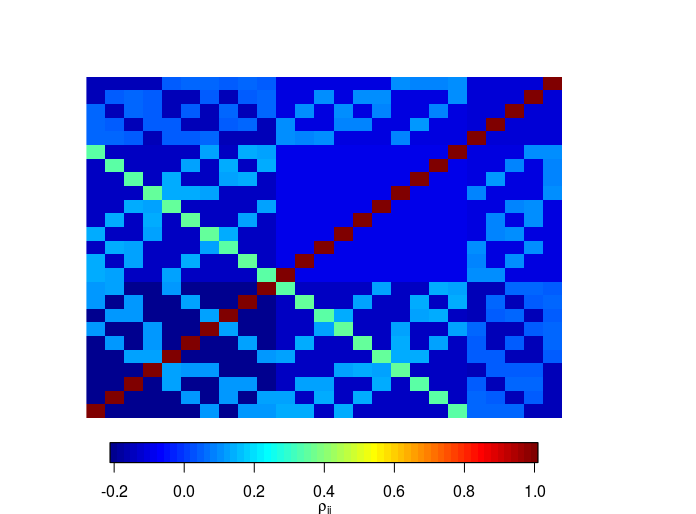
\includegraphics[scale=1]{\dir/figs/clade_corr.png} 
  \end{center}
\caption[Clade correlation matrix (coalescent prior), $n = 5$.]{\textbf{Clade correlation matrix (coalescent prior), $n = 5$}.
I sampled 10, 000 trees under the constant population size coalescent prior with contemporaneous tips using BEAST and computed the correlation matrix between clades of sizes between $2$ and $4$.
To facilitate visualisation of the structure in the matrix, I sorted clades by size (grows from bottom to top and left to right).
}
\label{fig:clade_corr}
\end{figure}


\subsection{Multi-dimensional scaling}
\label{sec:mds}

One way of visualising phylogenetic space is by employing lower-dimension projections that attempt to embed it in Euclidean space.
A very popular technique for this purpose is multi-dimensional scaling (MDS, \cite{Hillis2005}) of phylogenetic distances, in which the idea is to construct a new space with a few (usually two) dimensions that captures most of the features (variability) of the original space.
Suppose $\boldsymbol D$ is a phylogenetic distance matrix where $D_{ij}$ is the distance -- under a particular metric $d_\sigma$ -- between two  phylogenies $i$ and $j$.
MDS proceeds by finding points $\boldsymbol x = \{x_1, x_2, \ldots, x_P\}$ such that a~\textbf{stress function}~\citep{Kruskal1964}\footnote{Other stress functions are possible, I keep the Kruskal-1 function here for simplicity and comparability with~\cite{Hillis2005}.}:
\begin{equation}
 \label{eq:stressF}
 S_D(\boldsymbol x) =  \sqrt{ \sum_{i \neq j = 1}^P \left( D_{ij} - |x_i - x_j|\right)^2},
\end{equation}
is minimised.
As pointed out by~\cite{Hillis2005}, under certain conditions this ensures the new space does not contain large distortions from the distance matrix and hence the new space can be used as representation of phylogenetic space.
Once we have an optimal solution computed from the observed distances, $\boldsymbol x$, we can use it to produce visualisations.

While the original paper by~\cite{Hillis2005} employed Robinson-Foulds to compose $\boldsymbol D$,~\cite{Jombart2017} generalise that approach by developing an R package to aid MDS visualisation under different metrics, with special focus on the KC metric~\citep{Kendall2016}.
In addition,~\cite{Jombart2017} also provide ways of extracting representative trees from a large sample, which reflect median points around which trees cluster.
This might prove particularly useful when finding and characterising \textit{modes} in phylogenetic space.

In order to enable meaningful comparisons between runs, I employ the Procrustes method to obtain an optimal rotation/scaling of the resulting distance matrices such that they are as compatible as possible. 
This helps minimise distortions caused by stochastic variation and allows MDS projections from different sets of phylogenies to be overlaid for comparison.
I used the function \verb|procrustes()| from the R package \textbf{vegan}~\citep{Oksanen2018} to obtain Procrustes-transformed matrices.

\textbf{Limitations}

As noted in Section 3 of~\cite{Willis2017}, phylogenetic space cannot be completely embedded in Euclidean space, hence any procedure that produces a mapping $\boldsymbol\Phi \to \mathbb{R}^P$ will invariably lead to the loss of some information.
A comprehensive assessment of the relative merits of different stress functions and phylogenetic metrics is lacking, and unfortunately outside the scope of this chapter.
Moreover, since 2-d visualisations are so much easier to understand, practitioners might be tempted to only consider the first two coordinates of the transformed space, what might in turn lead to missing important features in the data.

\subsection{Graph (network) analysis of tree space}
\label{sec:graph}

Another useful way of representing the discrete (tree) component of phylogenetic space is equipping it with a metric $d_\sigma$ and constructing a graph $G_\delta(V_n, E_n)$ where each vertex corresponds to a tree topology and there is an edge between two edges (trees) if they are a distance $d_\sigma \leq \delta$ apart under the chosen metric.
Thus, for this ``meta-graph'', $|V_n| = |\mathbb{F}| = (2n-3)!!$ and $|E_n| \leq |V_n| (|V_n| - 1)/2$, although this last bound is very crude and can be refined for a given $d$ and $\delta$.
Common choices for metric include the nearest-neighbour interchange (NNI) and subtree prune-and-regraft (SPR) distances.
In particular,~\cite{Whidden2015} show how one can construct the SPR graph of a sample of trees and then use graph-theoretic tools to quantify exploration of phylogenetic space. 
Starting from a sample of trees $\boldsymbol \tau = \{\tau_1, \tau_2, \ldots, \tau_M\}$, the analysis pipeline proposed by~\cite{Whidden2015} can be summarised as follows:
\begin{enumerate}
 \setcounter{enumi}{-1} 
 \item Rank the elements in $\boldsymbol\tau$ by their posterior probability (frequency), creating a set $\boldsymbol \tau_{\text{top}}$, also determine the most probable tree, $\tau_{\text{max}}$;
 \item Keep only the $m = \text{min}(4096, |\boldsymbol\tau_{\text{top}}|)$ first elements;
 \item Compute the $m \times m$ matrix of SPR distances between the samples, $\boldsymbol D$, and construct a graph $\boldsymbol G$ where each tree is a vertex and two vertices $i$ and $j$ are connected by an edge if $D_{ij} = 1$, that is, if the two phylogenies are one SPR operation apart from each other;
 \item Identify clusters of high-probability trees by iteratively clustering trees until $K=8$ clusters are obtained;
 \item Visualise the resulting graph annotating the vertices with posterior probabilities and distance to the most probable (or mode) tree. 
\end{enumerate}

~\cite{Whidden2015} also propose three metrics -- which can all be computed with a single pass on $\boldsymbol\tau_{\text{top}}$ -- to quantify exploration of tree space:
\begin{enumerate}
 \item Mean access time (MAT): average number of iterations required to visit any two trees;
 \item Mean commute time (MCT): average number of iterations required to go from $\boldsymbol \tau_{\text{top}}$ to each of the other high probability trees and back;
 \item Round-trip cover time: starting from $\tau_{\text{max}}$, the average number of iterations necessary to visit each high probability tree and then return to the mode tree. 
\end{enumerate}

\textbf{Limitations}

One of the advantages of building $\boldsymbol G$ using SPR distances is that many of its theoretical properties are better studied~\citep{Whidden2017}.
On the other hand, focussing on SPR distances disregards branch lengths, which is not always desirable, specially when dealing with time-calibrated phylogenies (see below).
Perhaps a more serious flaw with the SPR-graph approach is that for large $n$,  each tree visited in the MCMC is likely to be unique, and hence one cannot construct $\boldsymbol \tau_{\text{top}}$ based on posterior frequencies.

\subsection{Effective sample size and potential scale reduction factor for phylogenies}
\label{sec:treeESS}

Recently, researchers have also extended the concepts of effective sample size (ESS) and potential scale reduction factor (PSRF) to tree topologies, taking advantage of the fact that these quantities are defined w.r.t. the L$^2$ in Euclidean space.
\cite{Lanfear2016} propose two ESS-like metrics:  (i) the \textbf{pseudo-ESS}, $n_{\text{eff}}^P$ and (ii) the topological \textbf{approximate ESS}, $n_{\text{eff}}^T$.
If we define $\tau_f$ to be a focal tree and let $\boldsymbol L = \{l_1, l_2, \ldots, l_M \}, \: l_i = d_\sigma(\tau_i, \tau_f)$, the pseudo-ESS is simply the ESS of $\boldsymbol L$  computed as defined above (Eq~\ref{eq:ESSb}).
In other words, this measure attempts to reduce phylogenies to a univariate continuous quantity for which the methods discussed in Section~\ref{sec:continuous} can be applied.
An advantage of this approach is that it admits any choice of metric $d_\sigma$, which in turn means one can use metrics that account for branch lengths and topology simultaneously.
A perhaps more principled approach is to try to directly estimate the autocorrelation spectrum for phylogenies.
Let $d$ be the squared distance between two independent phylogenies.
The expected value of $d$ with $N$ independent samples is $(N(N-1)/4N^2)d$ and we can estimate $N$ (as $n_{\text{eff}}^T$) when our sample has $M$ sequential observations by noting that 
\begin{align}
\label{eq:topoApproxESS}
\frac{N(N-1)}{4N^2} = \frac{\sum_{i = 1}^{M-1} \sum_{k = 1}^{\text{min}(m, M-i)}f(k)  + \frac{1}{2}(M-m + 1)(M-m)d}{2M^2},&\\
N = \left[\frac{2\sum_{i = 1}^{M-1} \sum_{k = 1}^{\text{min}(m, M-i)}f(k)  + (M-m + 1)(M-m)d - M^2}{M^2}\right]^{-1},&
\end{align}
where $f(k)$ is the squared distance between two samples at sampling interval (lag) $k$ and $m$ is the minimum sampling interval at which any two samples are independent,~\textit{i.e.}, the point where the autocorrelation function reaches an asymptote.  
\cite{Lanfear2016} suggest using an exponential model to estimate the autocorrelations, $f_a(k) = d(1-\exp(k/a))$, where $a$ is a shape parameter.
Implementations of both these functions are available in the \textbf{RWTY} package~\citep{Warren2017}.

The idea of treating squared distances as a surrogate for variance as employed above can be further extended to compute a PSRF-like for multiple samples of phylogenies.
\cite{Whidden2015} propose a ``topological Gelman--Rubin-like convergence diagnostic'', $\hat{R}^\prime$, that is very similar to~(\ref{eq:PRSF}) with $B$ and $W$ replaced by:
\begin{align}
 W^\prime &= \left(M(M-1)\right)^{-1}\sum_{k =1}^K\sum_{j_1 = 1}^M\sum_{j_2 = 1}^M d_\sigma(\tau_{kj_1}, \tau_{kj_2})^2,\\
 B^\prime &= \left((K-1)KM^2\right)^{-1} \sum_{i_1 = 1}^K\sum_{i_2 = 1}^K\sum_{j_1 = 1}^M \sum_{j_2 = 1}^M d_\sigma(\tau_{i_1j_1}, \tau_{i_2j_2})^2,\: \text{hence}\\
 \label{eq:PSRF-phylo}
 \hat{R}^\prime &= \sqrt{\frac{ (M-1)W^\prime +  B^\prime }{MW^\prime}}.
\end{align}
As with the original PSRF, $\hat{R}^\prime$ approaches 1 as the $K$ independent runs converge, and $\hat{R}^\prime < 1.1$ cut-off for convergence could be adopted.

\textbf{Limitations}

According to~\cite{Lanfear2016}, the pseudo-ESS can be sensitive to the choice of focal tree.
While that could be remedied in principle by choosing, for instance, the maximum clade credibility (MCC) phylogeny as $\tau_f$, it is unclear to me what biases this could introduce.
The original formulation of~(\ref{eq:PSRF-phylo}) by~\cite{Whidden2015} considered only SPR distances, but this can be easily generalised to other distances that include branch lengths.
A minor point about these diagnostics is that due to their recent development, in-depth theoretical and empirical studies are still lacking.
For instance, the choice of metric might play an important role in the power to detect convergence problems, but this aspect remains to be investigated.

\subsection{A word of caution}

As Charlie Geyer points out in the very quaintly named web page ``On the Bogosity of MCMC Diagnostics''\footnote{Available from \url{http://users.stat.umn.edu/~geyer/mcmc/diag.html}, accessed on 2018-02-18.}, all known diagnostic measures
%-- barring perhaps the so-called ``perfect sampling'' method~\citep{Propp1996} --
have serious shortcomings and, in his words, can detect only ``... obvious, gross, embarrassing problems that jump out of simple plots''.
While I do not completely subscribe to Geyer's view,  I agree that subtle problems such as small biases in the Hastings ratio (see e.g.~\cite{Holder2005}) or funnel-like effects of posterior (prior) correlation are likely to remain undetected.
Therefore a word of caution is warranted: even when one fails to detect convergence problems~\citep{Cowles1999}, they may very well still be present in the form of subtle biases, the impact of which on inferences drawn from the MCMC samples is hard to predict.

\section{Accommodating time-calibrated phylogenies}
\label{sec:accommodating}

In this Chapter I provide a first attempt at an unified workflow for Bayesian estimation of time-calibrated phylogenies (TCPs) with special focus on phylodynamic inference.
As discussed previously, TCPs are special objects in that the branch lengths are measured in units of calendar time.
In what follows I detail my investigations into several issues related to accommodating time-calibrated phylogenies and diagnosing the convergence of MCMC runs from BEAST.
Considering the methods currently available, the main difficulties faced when exploring the space of TCPs are:
\begin{itemize}
 \item Size: the phylogenies used in phylodynamic studies have $n$ of the order of hundreds to a few thousands (see below);
 \item Branch lengths: in time-calibrated phylogenies branch lengths are of crucial importance and hence cannot be ignored;
 \item Sampling structure: TCPs usually have serially-sampled tips/leaves.
 The distribution and range of the sampling times imposes constraints on the phylogenetic space, leading to ``rugged'' posterior distributions~\citep{Brown2018} -- see also Figure 3. in~\cite{Moller2018} and discussion therein. 
\end{itemize}

Most routines in AWTY are designed for unrooted trees and implicitly assume a relatively small number of taxa ($n < 50$).
Moreover, the MDS routines presented in~\cite{Hillis2005} and available in the~\textbf{RWTY} package use the Robinson-Foulds distance which does not capture branch length differences and hence is not appropriate for time-calibrated phylogenies if used in isolation.
The routines available in the~\textbf{RWTY} package also use RF as the default metric, and as far I am aware, the only metric that includes branch lengths available in the package is path distance (BS, see Section~\ref{sec:metrics}).
Here I relax this by including many other metrics (see below), for which the approximate ESS of~\cite{Lanfear2016} can be computed using equation~(\ref{eq:topoApproxESS}).
As the number of taxa grows, it gets progressively harder to track clades, both from a statistical and a computational point of view.
Computationally, it becomes cumbersome to compute indicators for all clades in a run, in addition to plotting clade frequencies.
This latter problem can be tackled by only paying attention to clades with a particular (posterior) frequency.
Statistically, however, the space of clades presents some non-trivial correlation structure that might make it hard to obtain reliable global indicators of convergence and mixing.
In Section~\ref{sec:cladeSwitch}, I provide a more detailed discussion of these issues.
Nonetheless, in the interest of consistence and comparability with previous approaches I include diagnostics of convergence and mixing in clade space. 

In a phylodynamic analysis context one may be chiefly interested in a set $\boldsymbol\theta^\star$ parameters, which might include quantities such as the reproductive ratio $R_0$~\citep{Stadler2011} or the wave front velocity of an epidemic~\citep{Lemey2010,Pybus2012}.
It is therefore important to study the behaviour of the chains for $\boldsymbol\theta^\star$, as well as account for the correlations between parameters.
Fortunately, there are a plethora of tools designed to diagnose convergence for continuous parameters, many of which are available in the R package~\textbf{coda}~\citep{Plummer2006} and the GUI application Tracer~\citep{Rambaut2018}.

The pipeline/workflow proposed here can be summarised as follows:
\begin{enumerate}
 \item Run (at least) three independent chains for $M$ iterations each, keeping $M_t$ phylogenies;
 \item Compute univariate ESS, PSRF and mESS for $\boldsymbol\theta^\star$;
 \item (Sub)sample a number $K < M_t$ of trees and compute ($ K \times K$) distance matrices under different metrics;
 \item Perform MDS on the distance matrices and use them to visualise phylogenetic space (see Figure~\ref{fig:pipeline}b);
 \item Using the same distance matrices, compute the approximate ESS~\citep{Lanfear2016} for each run under different metrics;
 \item Compute clade frequencies and indicator matrices and calculate clade ESS, clade switching and average standard deviation in split/clade frequencies (ASDSF);
\end{enumerate}

\subsection*{Specialised computer programs}

Most modern phylodynamic studies include data sets with hundreds to a few thousands of samples (taxa) and the resulting phylogenies strain the capacity of most existing packages (including AWTY and RWTY).
Computationally, one of the main bottlenecks is loading trees into memory -- which is quite slow in R, for instance.
I instead do the tree-processing externally using specialised classes in BEAST (\verb|dr.app.tools.TopologyTracer|)\footnote{Implemented by Andrew Rambaut and Guy Baele (Leuven) with input and testing from me.}, controlled using simple bash scripts.
I then wrote custom R functions to transform the output of \verb|TopologyTracer| so that it could be analysed using heavily modified functions in the package~\textbf{RWTY}~\cite{Warren2017}.
The same strategy can be adopted when processing clade frequencies: I used the class \verb|dr.app.tools.TreeSummary| to compute clade frequencies and construct the indicator matrix and then modified functions from the \textbf{RWTY} package for plotting and presenting the results.
As mentioned above, I employ the packages~\textbf{mcmse}~\citep{Flegal2017} and~\textbf{coda}~\citep{Plummer2006} to compute (univariate and multivariate) effective sample sizes and potential scale reduction factors for continuous parameters.
This is done to keep all computations contained in the R environment, which allows the whole workflow to be encapsulated into a (R)Markdown document which can be rendered to html and/or PDF (see Figure~\ref{fig:pipeline}).
A suite of R and bash scripts -- as well as the RMarkdown report --  to perform these tasks is available from~\url{https://github.com/maxbiostat/BEAST_convergence_pipeline}\footnote{If these functions prove to be sufficiently useful to other researchers, I may build an R package.}.
For convenience, the analysis of the ``poor'' runs (see below) is included in Appendix A as an example.
\begin{figure}[!ht]
\begin{center}
  \subfigure[\textbf{Continuous parameters}]{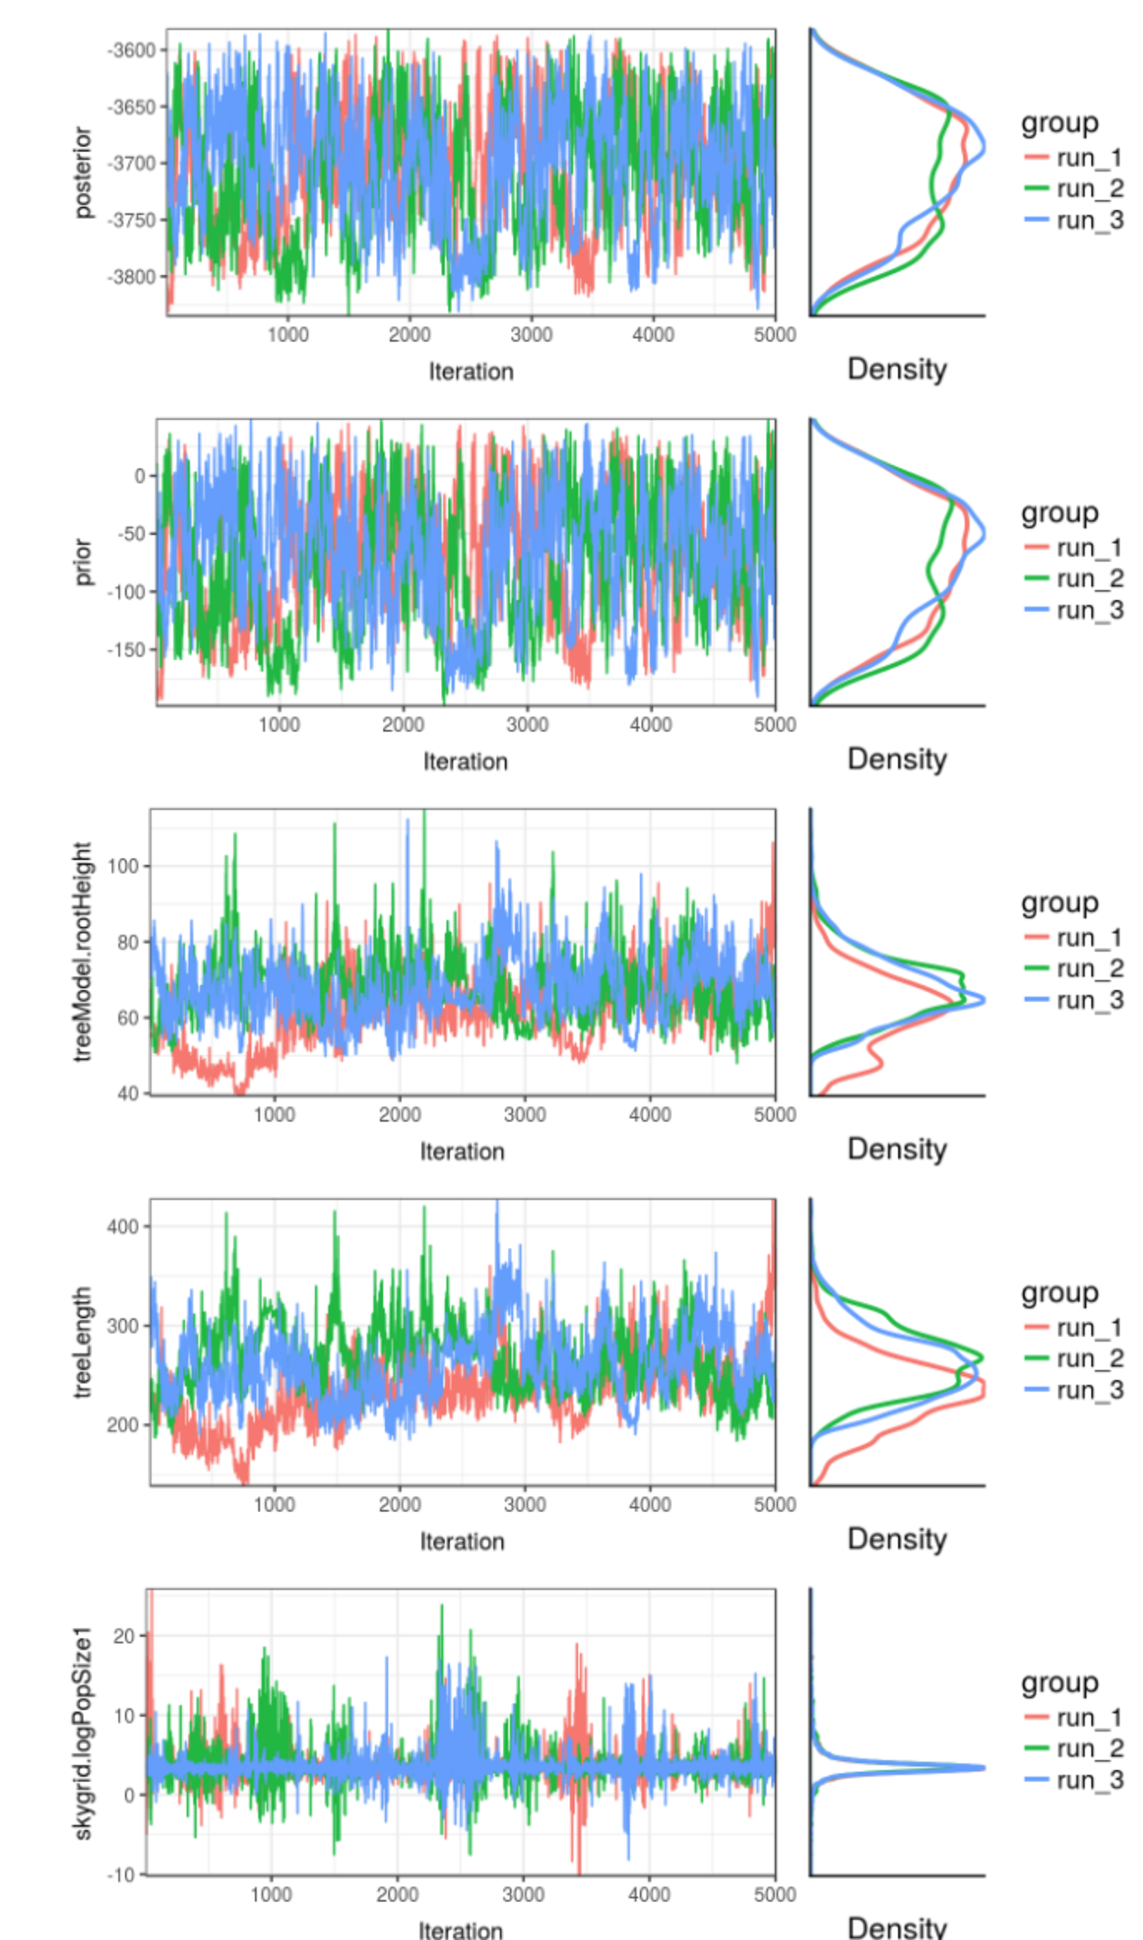
\includegraphics[scale=0.35]{\dir/figs/pipeline_screenshot.pdf}}%
  \subfigure[\textbf{MDS}]{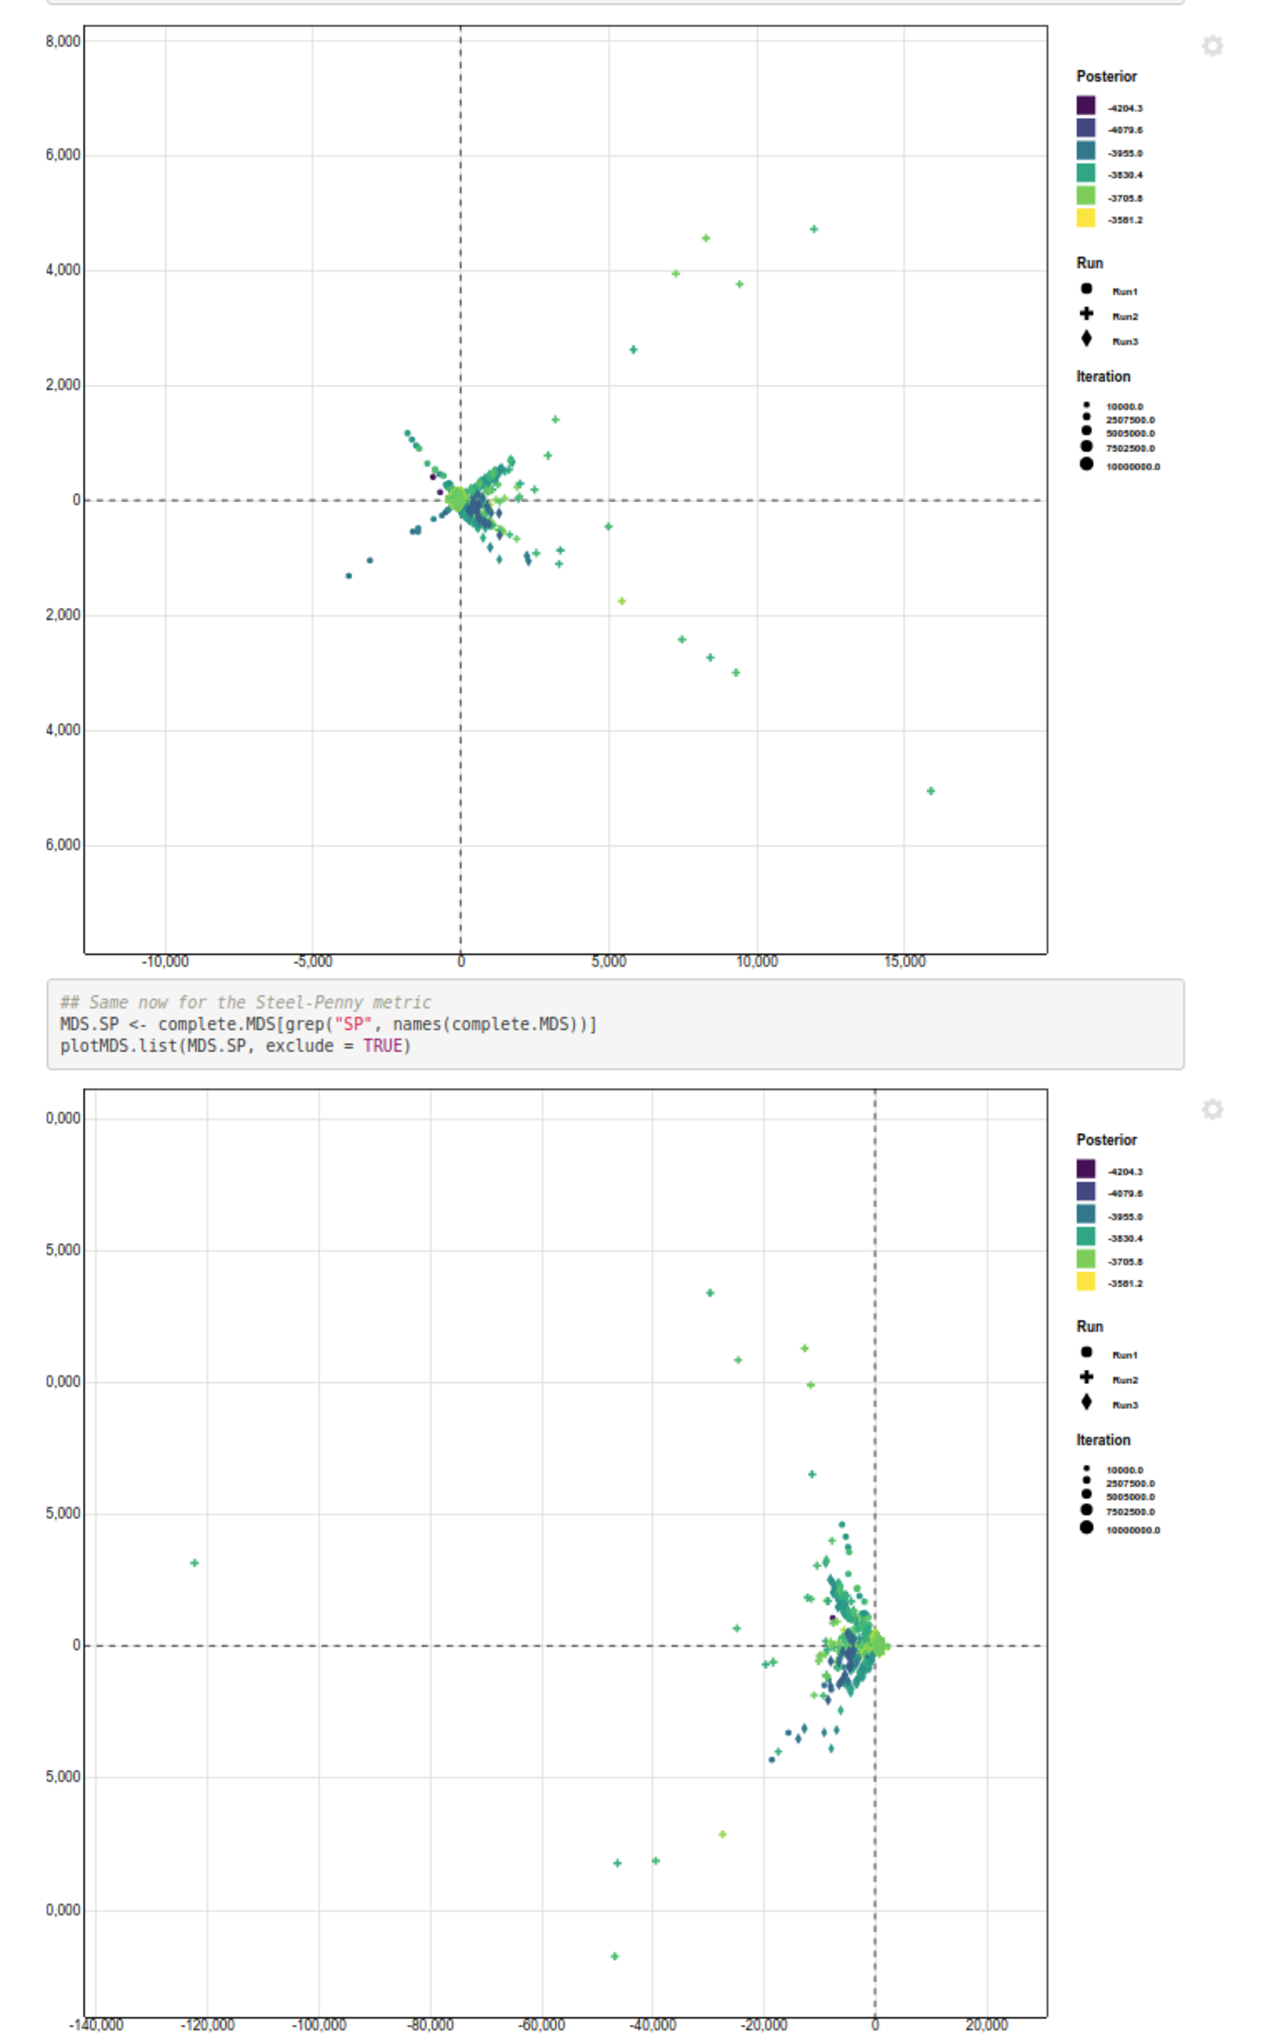
\includegraphics[scale=0.35]{\dir/figs/pipeline_screenshot_mds.pdf} } 
\end{center}
 \caption[Screen capture of the proposed MCMC diagnostics pipeline.]{\textbf{Screen capture of the proposed MCMC diagnostics pipeline}.
One can check  trace plots -- as well as investigate univariate and multivariate ESS -- for continuous parameters (a) and study exploration of phylogenetic space by visualising MDS (b) -- note these latter plots are made interactive  using the spreadD3() function in R.
All routines have been written in R and organised into an RMarkdown document that generates an html report that can easily explored by the user to diagnose problems with her MCMC runs.
See Appendix A for more.
 }
 \label{fig:pipeline}
\end{figure}

\section{Data sets}
\label{sec:data}

Here I will analyse the same data sets described in Table~\ref{tab:datasets} in Chapter 2.
In particular, \verb|Dengue4|, due to its manageable size but relatively high complexity (multiple partitions, temporal structure, etc), will be used to exemplify the full breadth of convergence diagnostics available and how they may be combined for maximum efficacy.
I will analyse MCMC runs resulting from empirical analyses of these data sets to investigate the characteristics of phylogenetic space for serially-sampled data modelled under phylodynamic models.
For the results in Section~\ref{sec:combining}, I constructed a deliberately bad MCMC sampler to obtain a poorly mixing chain.
To achieve this I employed only the \verb|WideExchange| operator  -- with small weight -- to sample tree topologies.
Since this operator is not "tunable" and has a very low acceptance probability ($0.021$ for this data set), the chain mixes poorly.
These poorly mixing (Poor) runs were then compared with runs using the default settings in BEAUti, the GUI configuration file maker for BEAST.
In addition, I ran the pipeline with \verb|STL| replacing all tree-related operators with the \verb|SubTreeLeap| operator described in Chapter 2.
All runs had 10 million iterations and a thinning interval of a thousand states. 

\subsection{Simulated data}
\label{sec:simudata}

I also created a simulated data set in order to have a baseline where we know the ground truth.
I first obtained a 50 taxa subtree with uniformly temporally sampled tips from a larger EBOV phylogeny~\citep{Dudas2017}, henceforth called ``empirical tree''.
To assess the effect of tree shape, I simulated a coalescent tree with the same tip-date sampling structure under a constant population model with $N_e = 10$, which I will call ``coalescent tree''.
I then simulated alignments of 1,000, 5,000 and 10,000 sites down both trees with a substitution rate of $10^{-3}$ substitutions per site per year, generating 6 alignments.
For each alignment, I then ran three independent runs (replicates) of both STL and the default/classic mix.
To explore convergence times and obtain more stable estimates of the posterior, each combination of data set and transition kernels was run 10 million and 100 million iterations.

\section{Analysis}
\label{sec:results}

\subsection{Combining diagnostic measures}
\label{sec:combining}

The first set of results I will present is the development of an analysis ``pipeline'' for MCMC diagnostics in Bayesian phylogenetics.
In particular, I will use the Dengue serotype 4 \textit{env} (\verb|Dengue4|) -- 17 taxa, 1485 sites -- to showcase how many convergence diagnostic measures can be employed in conjunction as part of the Bayesian phylogenetic workflow.
Appendix A shows the analysis of the poorly mixing runs using the steps and computer programs described above.
In this section I focus on comparing some results for three MCMC schemes: poorly mixing, default settings and \verb|STL|.

First, I present the results of convergence diagnostics for continuous parameters, usually obtained with the graphical tool Tracer in the context of BEAST analyses.
Here however I compute some additional quantities not available in Tracer, such as multivariate ESS and potential scale reduction factor (PSRF).
Results in Table~\ref{tab:continuous_results} show that the poor runs have low univariate ESSs for continuous parameters highly dependent on the tree (e.g., mean evolutionary rate, \verb|meanRate|), whereas ESS are in the low thousands for parameters such as the transition transversion rate ($\kappa$).
For this particular experiment and with no optimisation, \verb|STL| shows comparable if slightly inferior performance when comparing raw univariate ESSs.
The PSRFs show that for many of these parameters the three independent runs do not converge to the same point (PSRF $> 1.1$), be it individually for each parameter or globally across parameters (multivariate PSRF $> 1.1$).
While the \verb|STL| runs seem more consistent, as indicated by the slightly lower PSRFs, with only three runs (chains) per MCMC scheme this difference cannot be reliably established (see Chapter 2 for more thorough comparisons).
The multivariate ESSs might at first glance give the impression of good performance, but in fact all of them fall well short of the minimum ESS required for reliable inference (see caption in Table~\ref{tab:continuous_results}).
Notice that while this is specially the case for the poor runs (as expected), none of the runs across MCMC schemes achieve the minimum ESS (8831) after 10 million iterations (see Discussion).

\begin{sidewaystable}[!ht]
\caption[Convergence diagnostics for continuous parameters.]{\textbf{Convergence diagnostics for continuous parameters}.
I show the summary convergence diagnostics from the pipeline described in Section~\ref{sec:accommodating} for three MCMC schemes, running three chains for each.
$^1$ - First (log) population  from Skygrid.
$^2$ - The ratio between the average rate and the standard deviation of rates across all branches.
$^3$ - Covariance between rate assignments in the tree.
$^4$ - Multivariate ESS as in~\cite{Vats2015} and multivariate potential scale reduction factor (PSRF).
The minimum multivariate ESS for all parameters considered should be $8831$ according to the formula in~(\ref{eq:mESSbound}).
}
\label{tab:continuous_results}
\begin{center}
\small\addtolength{\tabcolsep}{-5pt}
 \begin{tabular}{ccccc|cccc|cccc}
\toprule
                         & \multicolumn{4}{c}{Poor}                  & \multicolumn{4}{c}{Default}               & \multicolumn{4}{c}{STL}                   \\
\midrule                         
Parameter                & ESS 1 & ESS 2 & ESS 3 & PSRF        & ESS 1 & ESS 2 & ESS 3 & PSRF        & ESS 1 & ESS 2 & ESS 3 & PSRF        \\
\midrule
Tree height              & 57      & 40      & 13      & 1.11 (1.33) & 1063    & 1113    & 876     & 1.03 (1.10) & 858     & 937     & 940     & 1.00 (1.01) \\
Tree length              & 55      & 34      & 7       & 1.17 (1.49) & 1021    & 1150    & 907     & 1.03 (1.10) & 860     & 1373    & 907     & 1.00 (1.01) \\
(log) Pop Size$^1$           & 622     & 657     & 27      & 1.01 (1.02) & 1098    & 833     & 751     & 1.00 (1.01) & 230     & 1138    & 1261    & 1.02 (1.03) \\
CP1.alpha                & 7446    & 6992    & 7202    & 1.00 (1.00) & 2705    & 2659    & 2484    & 1.00 (1.01) & 3567    & 3377    & 3320    & 1.00 (1.00) \\
CP1.kappa                & 8620    & 8695    & 8640    & 1.00 (1.00) & 4360    & 3796    & 3753    & 1.05 (1.07) & 5204    & 5551    & 4912    & 1.00 (1.00) \\
CP2.kappa                & 6763    & 6876    & 7325    & 1.00 (1.00) & 2674    & 2807    & 1983    & 1.00 (1.01) & 3255    & 3761    & 3571    & 1.00 (1.00) \\
Mean rate                & 46      & 49      & 12      & 1.17 (1.49) & 1058    & 1270    & 846     & 1.00 (1.00) & 741     & 1396    & 1002    & 1.00 (1.01) \\
Coefficient of variation$^2$ & 26      & 41      & 7       & 1.12 (1.28) & 748     & 794     & 817     & 1.00 (1.00) & 531     & 1147    & 1178    & 1.01 (1.02) \\
Covariance$^3$               & 3370    & 3370    & 1315    & 1.00 (1.00) & 5168    & 5209    & 5134    & 1.00 (1.00) & 6148    & 6088    & 6124    & 1.00 (1.00) \\
Multivariate ESS/PSRF$^4$    & 1299    & 1212    & 937     & 1.13        & 2018    & 2170    & 2034    & 1.02        & 1808    & 2632    & 2407    & 1.01       \\
\bottomrule
\end{tabular}
\end{center}
\end{sidewaystable}

Considering mixing and convergence in phylogenetic space through the use of specially tailored diagnostics presented in Table~\ref{tab:tree_results}, shows that while the approximate ESS~\citep{Lanfear2016} does capture major differences in mixing, it is inconsistent, both within and between metrics.
As an example, take the tree ESS with the Steel-Penny (SP) metric for the Poor runs: for one of the chains, it achieves its maximum value of 1001, when it clearly cannot be the case that the sample comprised 1001 independent samples considering all available evidence.
The clade switching score (CSS) and mean ESS for clade indicators seem to discriminate well between the Poor runs and the default (and \verb|STL|) ones.
ASDSF is also above the common threshold of $0.10$ used for convergence~\citep{Ronquist2012}; \verb|STL| seems to lead to slightly better performance according to this metric.
\begin{sidewaystable}[!ht]
\begin{center}
 \centering
\caption[Convergence diagnostics in phylogenetic space.]{\textbf{Convergence diagnostics in phylogenetic space}.
I show convergence diagnostics specially tailored towards phylogenetic space, such as the approximate ESS of~\cite{Lanfear2016} (for various metrics), the average univariate ESS for clade indicators$^1$, the clade switching score$^2$ and the average standard deviation in split/clade frequencies$^3$.
Tree ESSs computed using a sample of $1001$ trees following the expression in~(\ref{eq:topoApproxESS}).
}
\label{tab:tree_results}
\begin{tabular}{cccc|ccc|ccc}
\toprule
                 & \multicolumn{3}{c}{Poor}    & \multicolumn{3}{c}{Default} & \multicolumn{3}{c}{STL}     \\
                 \midrule  
                 & Chain 1 & Chain 2 & Chain 3 & Chain 1 & Chain 2 & Chain 3 & Chain 1 & Chain 2 & Chain 3 \\
                 \midrule  
Tree ESS (KC, $\lambda = 0$)   & 33      & 38      & 39      & 743     & 1001    & 1001    & 523     & 734     & 465     \\
Tree ESS (KC, $\lambda = 1/2$) & 156     & 305     & 20      & 444     & 581     & 1001    & 292     & 231     & 445     \\
Tree ESS (KC, $\lambda = 1$)   & 139     & 395     & 19      & 371     & 705     & 711     & 276     & 276     & 1001    \\
Tree ESS (RF)    & 55      & 114     & 36      & 794     & 1001    & 801     & 695     & 624     & 787     \\
Tree ESS (SP)    & 66      & 1001    & 14      & 403     & 659     & 659     & 184     & 155     & 552     \\
Tree ESS (CD)    & 1001    & 431     &  87     & 1001    & 1001    & 1001    & 1001    & 1001    & 1001     \\
Tree ESS (BS)    & 212     &  259    &  25     & 260     & 445     & 675     & 232     & 241     & 340     \\
Mean clade ESS$^1$   & 874     & 917     & 837     & 7321    & 7446    & 7420    & 7506    & 7477    & 7428    \\
CSS$^2$              & 0.16    & 0.18    & 0.16    & 0.87    & 0.88    & 0.88    & 0.88    & 0.88    & 0.9     \\
ASDSF$^3$            & 0.18    & 0.39    & 0.29    & 0.08    & 0.09    & 0.04    & 0.05    & 0.03    & 0.04   \\
\bottomrule
\end{tabular}
\end{center}
\end{sidewaystable}

I now move on to explore some more specific questions about phylogenetic space and its representations.

\subsection{Representation of phylogenetic space under different metrics}
\label{sec:representation}

While multi-dimensional scaling can be useful for visualising phylogenetic space, the issue of which metric to employ remains.
Since each of the many available metrics captures distinct features, one has to analyse MDS projections under different metrics in order to have a better grasp of the geometry of phylogenetic space.
In Figure~\ref{fig:mds_ebov_RF} I show the MDS projection of Robinson-Foulds (RF) distances between MCMC samples for the large Ebola virus data set (\verb|EBOVa|) -- the analysis detailed in Chapter 2, see Figure~\ref{fig:ebovmultimod}. 
It is clear that run 3 for the \verb|STL| operator (see Chapter 2) is distinct from the others. 
In addition, one can see that the last samples of run 2 \verb|STL| (larger green points) are closer to the region visited by the default runs and \verb|STL| run 1.
These results show that the projection using the Robinson-Foulds capture important features of phylogenetic space, leading to clearly separated clusters of trees with different likelihoods.

\begin{figure}[!ht]
\begin{center}
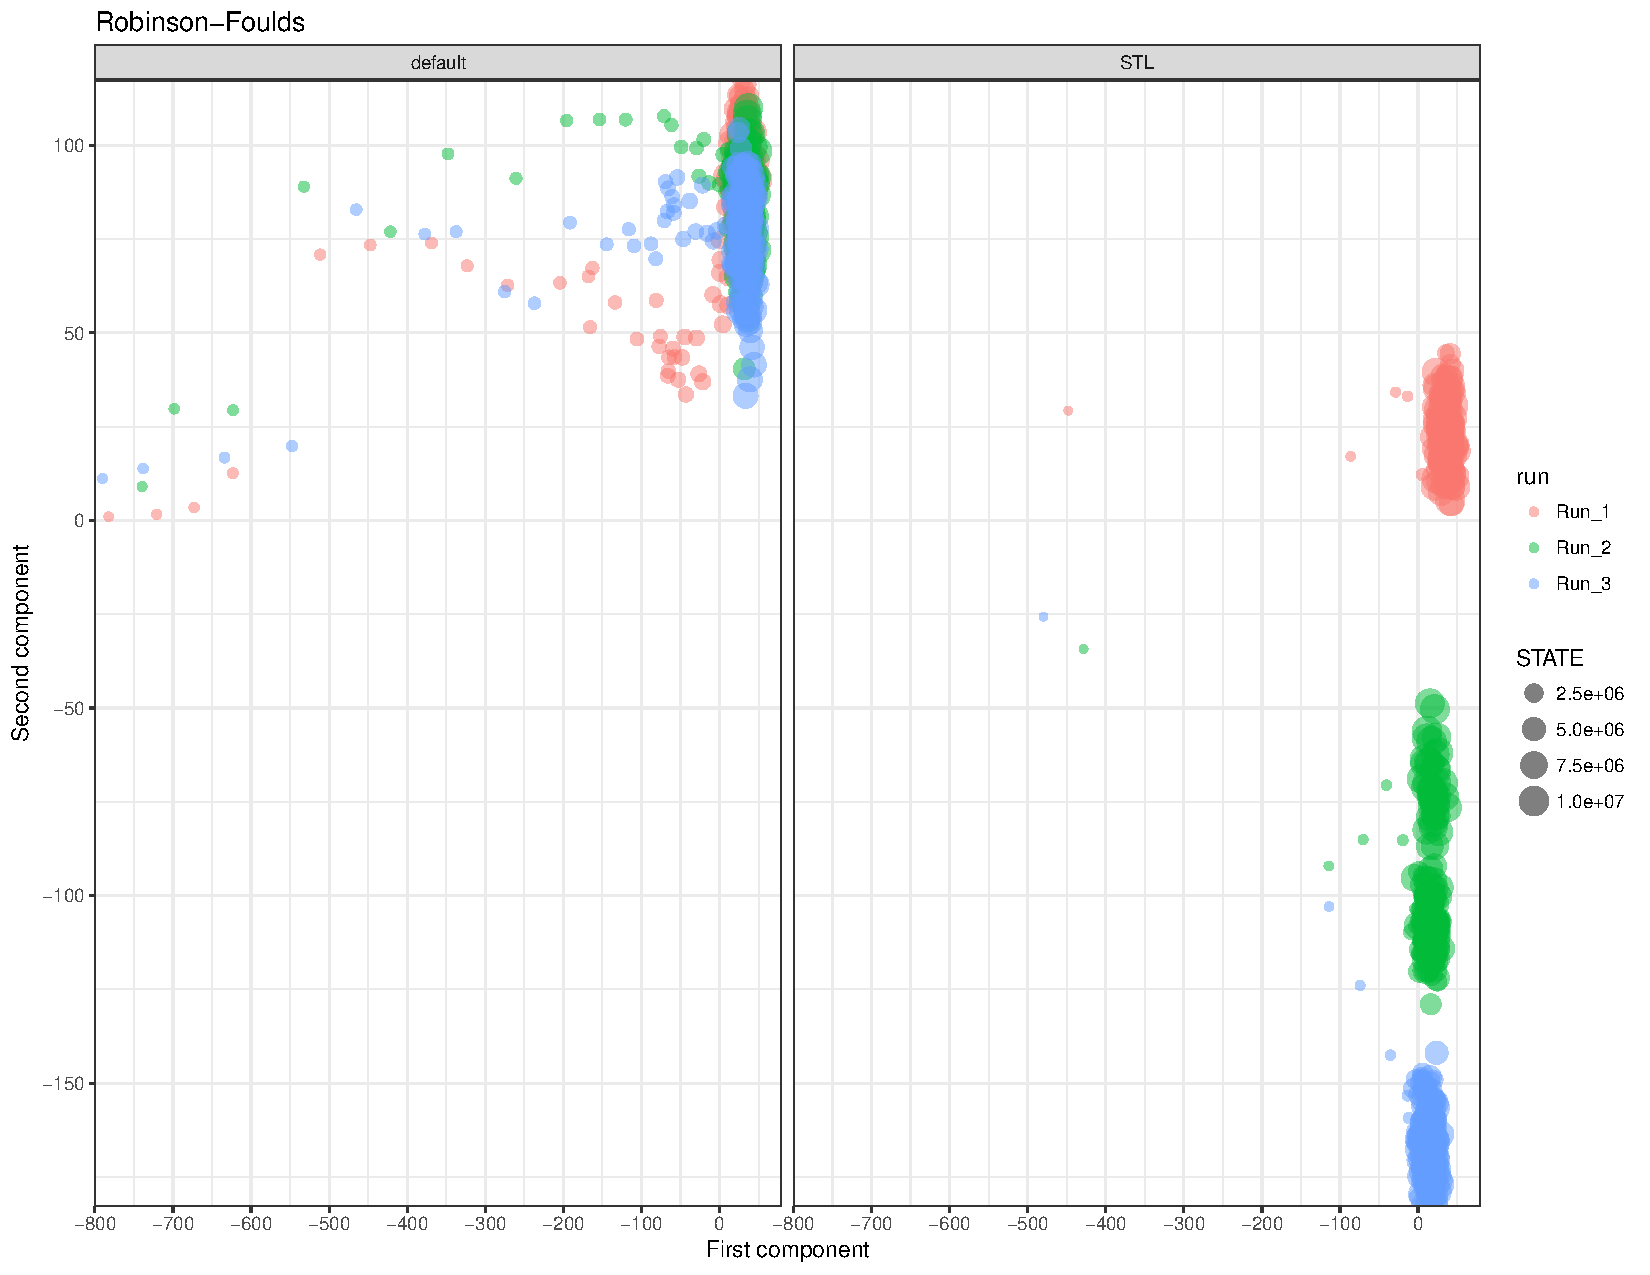
\includegraphics[scale=0.5]{\dir/figs/mds_ebov_RF.pdf} 
\end{center}
 \caption[MDS projections for the full EBOV 1610 taxa data set (Robinson-Foulds distances).]{\textbf{MDS projections for the full EBOV 1610 taxa data set (Robinson-Foulds distances).}
 I sampled 200  equally spaced trees from each chain (1200 trees in total) and computed the Robinson-Foulds distance~\citep{Robinson1981} for every pair of trees.
 Colours relate to the seed used in the pseudo random number generator, ensuring each run starts from the same point. 
 Please see Figure~\ref{fig:ebovmultimod} in Chapter 2 for more details. 
 The size (radius) of the dots is proportional to the state of the chain.
 }
 \label{fig:mds_ebov_RF}
\end{figure}

Importantly, however, these differences are not captured by other metrics.
The projections under the Kendall-Colijn  (KC) metric in Figure~\ref{fig:mds_ebov_KC} shows no obvious clustering of the runs, even though we know different runs explore trees with very different likelihoods.
In panel (a), I show the MDS projection of KC metric  with $\lambda = 0$, that considers only topological differences between phylogenies, but the projections do not show any obvious clustering of the runs, unlike the RF metric (Figure~\ref{fig:mds_ebov_RF}).
The projection with $\lambda = 1/2$ in panel (b) displays the same pattern.
This seems to suggest that MDS under this metric does not allow one to visualise the different modes in phylogenetic space, or, in other words, that KC is too smooth to capture the differences, at least for this data set.

\begin{figure}[!ht]
\begin{center}
\subfigure[$\lambda = 0$]{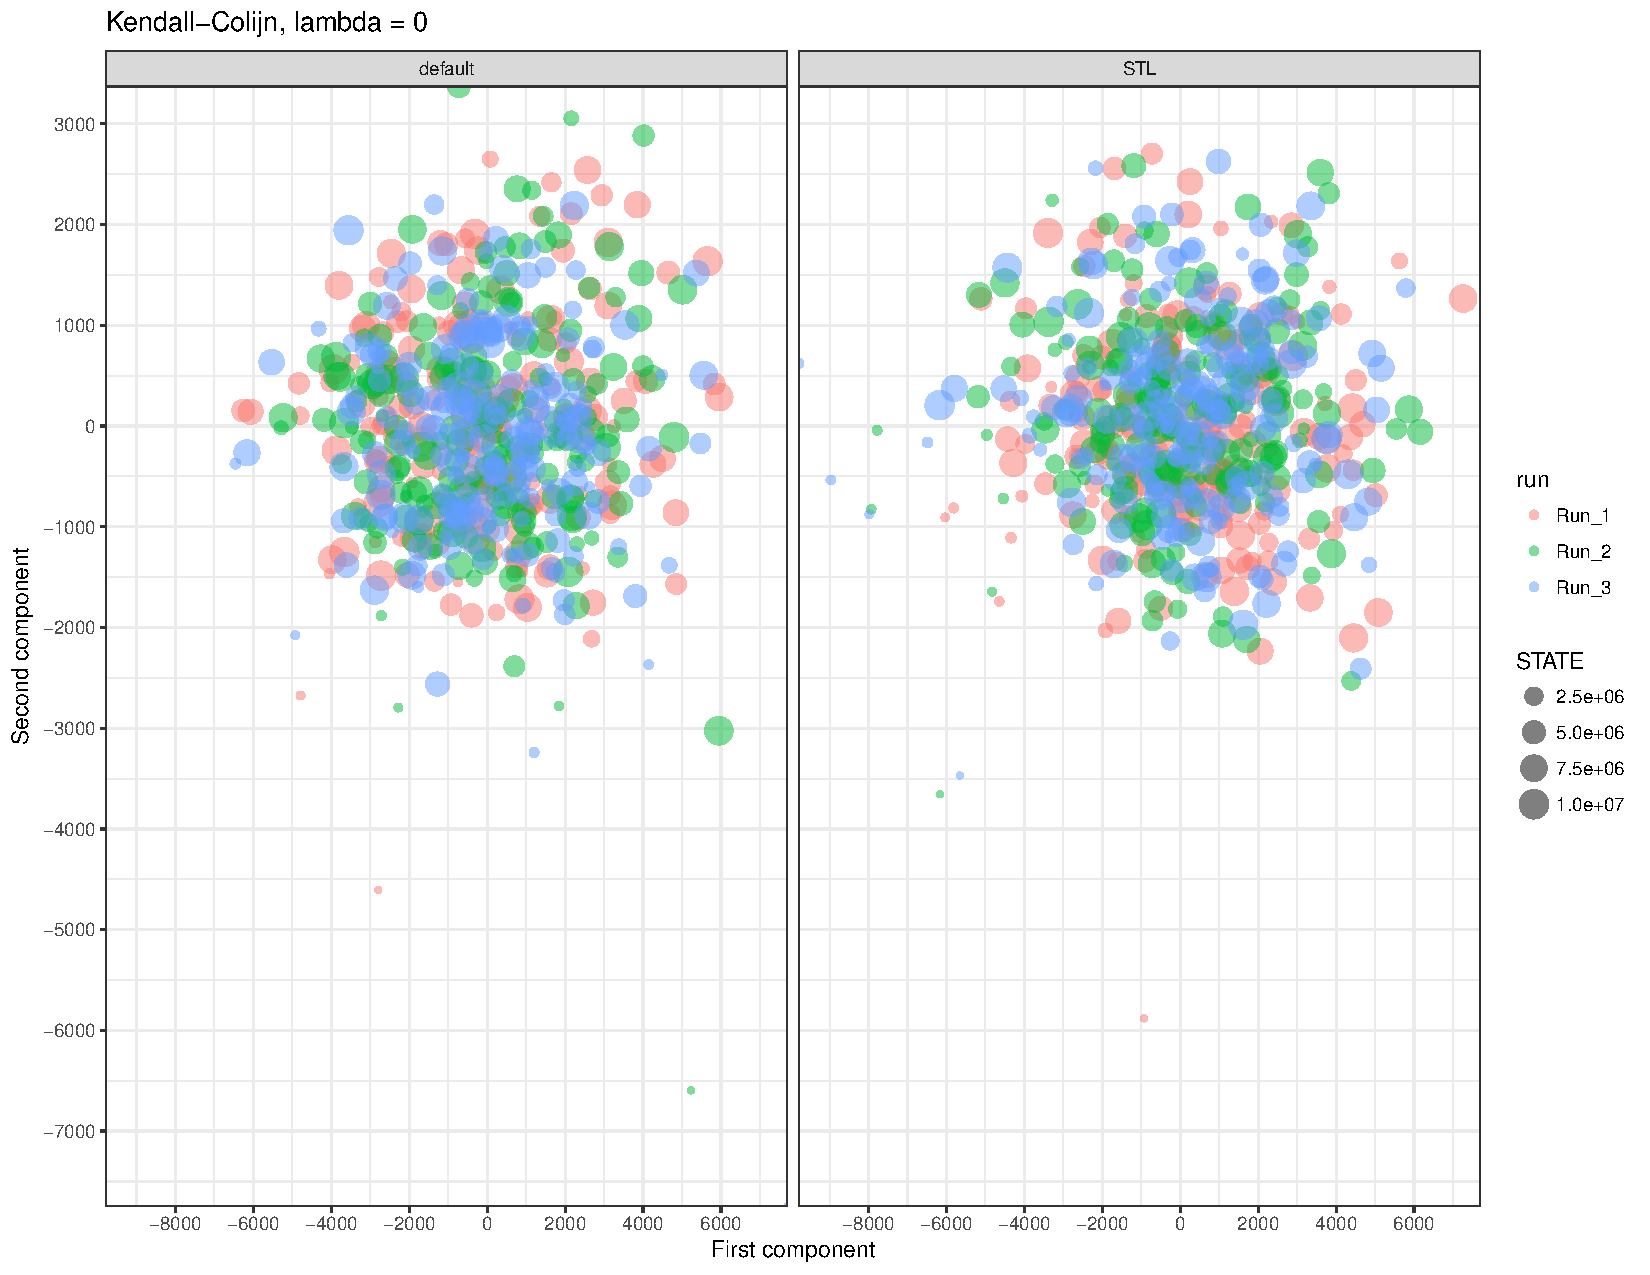
\includegraphics[scale=0.35]{\dir/figs/mds_ebov_KC0.pdf}}\\
\subfigure[$\lambda = 1/2$]{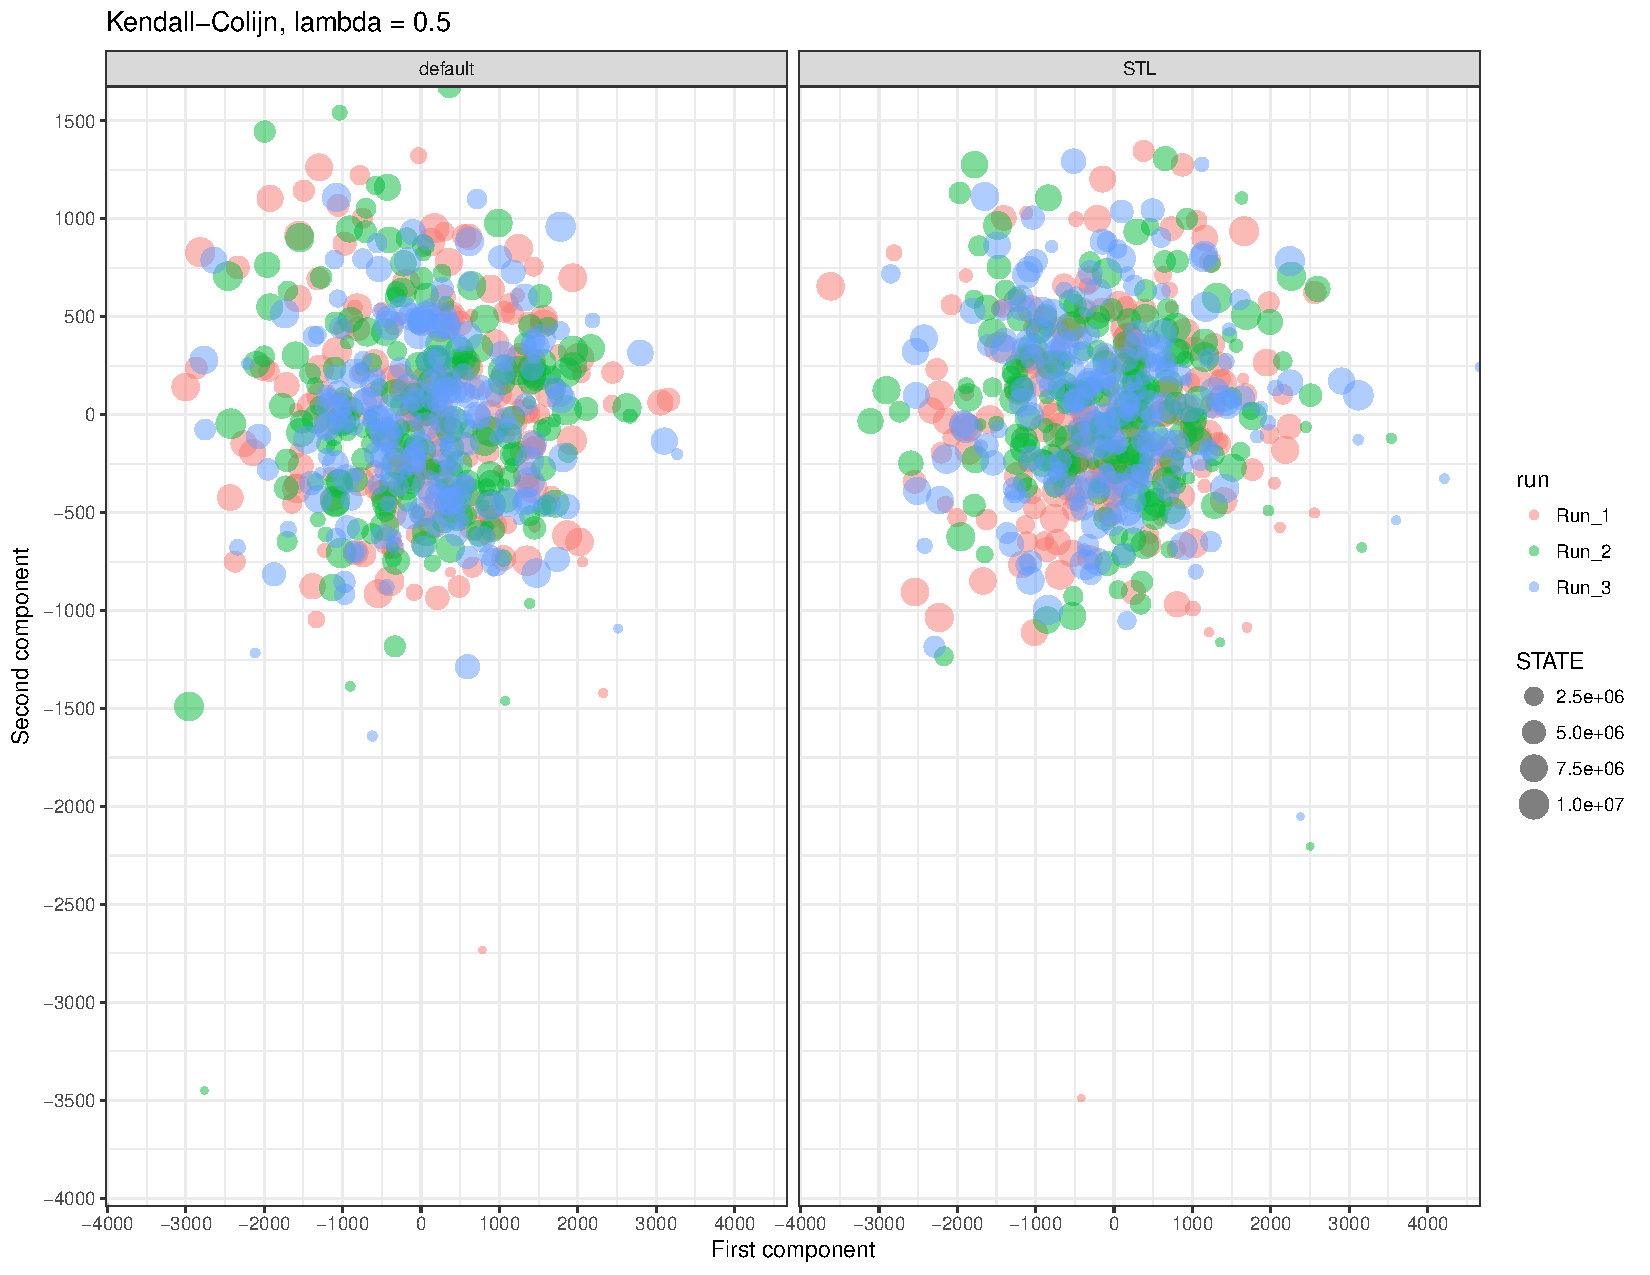
\includegraphics[scale=0.35]{\dir/figs/mds_ebov_KChalf.pdf}}
\end{center}
 \caption[MDS projections for the full EBOV 1610 taxa data set (Kendall-Colijn distances).]{\textbf{MDS projections for the full EBOV 1610 taxa data set (Kendall-Colijn distances).}
 I sampled 200 equally spaced trees from each chain (1200 trees in total) and computed the Kendall-Colijn distance with $\lambda = 0$ and $\lambda = 1/2$.
 Colours relate to the seed used in the pseudo random number generator, ensuring each run starts from the same point.  
 See Figure~\ref{fig:mds_ebov_RF} for the projection of the same trees under the Robinson-Foulds metric~\citep{Robinson1981}.
 }
 \label{fig:mds_ebov_KC}
\end{figure}

In Figure~\ref{fig:mds_ebov_SP} we can again notice the lack of differentiation between the runs, suggesting the SP metric shares the ``smoothness''  displayed by the KC metric.
Taken together, these results suggest that great care needs to be taken when visualising phylogenetic space because important features might not be easy to distinguish under many (most) metrics.

\begin{figure}[!ht]
\begin{center}
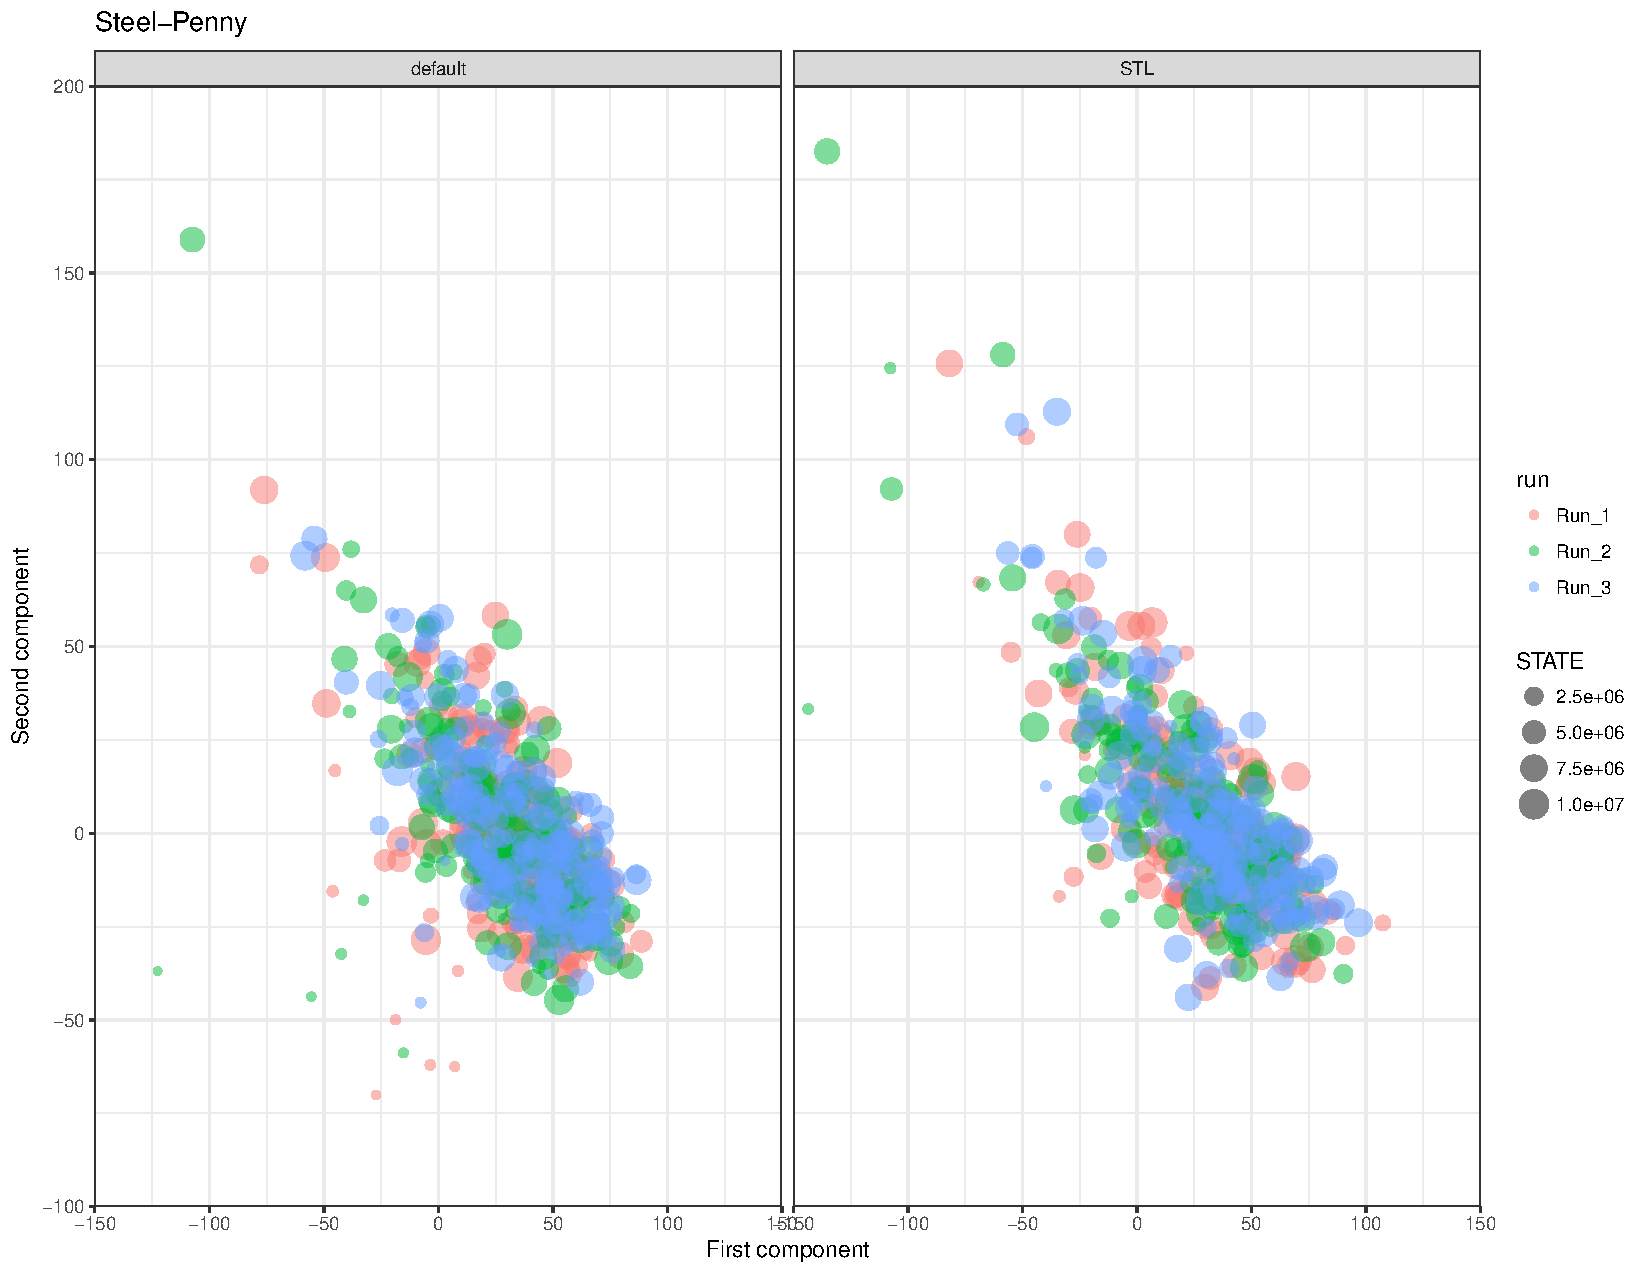
\includegraphics[scale=0.5]{\dir/figs/mds_ebov_SP.pdf} 
\end{center}
 \caption[MDS projections for the full EBOV 1610 taxa data set (Steel-Penny distances).]{\textbf{MDS projections for the full EBOV 1610 taxa data set (Steel-Penny distances).}
 I sampled 200  equally spaced trees from each chain (1200 trees in total) and computed the Steel-Penny distance~\citep{Steel1993} for every pair of trees.
 Colours relate to the seed used in the pseudo random number generator, ensuring each run starts from the same point. 
 See Figures~\ref{fig:mds_ebov_RF} and~\ref{fig:mds_ebov_KC} for projections of the same trees under different metrics.
 }
 \label{fig:mds_ebov_SP}
\end{figure}

One question seldom approached in the literature is the quality of MDS projections of phylogenetic space.
As mentioned above, it is standard practice to keep the first two components for plotting and analysis, but if this 2-d  projection is to be a faithful representation of the space of interest we need to ascertain that the first two components do indeed capture most of the variation.
A way of analysing the quality of the projections is to plot the scaled eigenvalues against the component number.
Ideally, the first few components capture most of the variation, resulting in an ``elbow-shaped'' plot.
In contrast, a flat plot suggests that variation is spread across many components and hence restricting attention to the first two can be misleading.
In Figure~\ref{fig:screeplots} I show these plots for a range of real-world data sets (see Table~\ref{tab:datasets} in Chapter 2).
A consistent result across data sets is the plot for the Robinson-Foulds (RF) distance, which is mostly flat and suggests that for this metric it is not sufficient to look at the first few components in order to get a good picture of the variation in the sample.

\begin{figure}[!ht]
\begin{center}
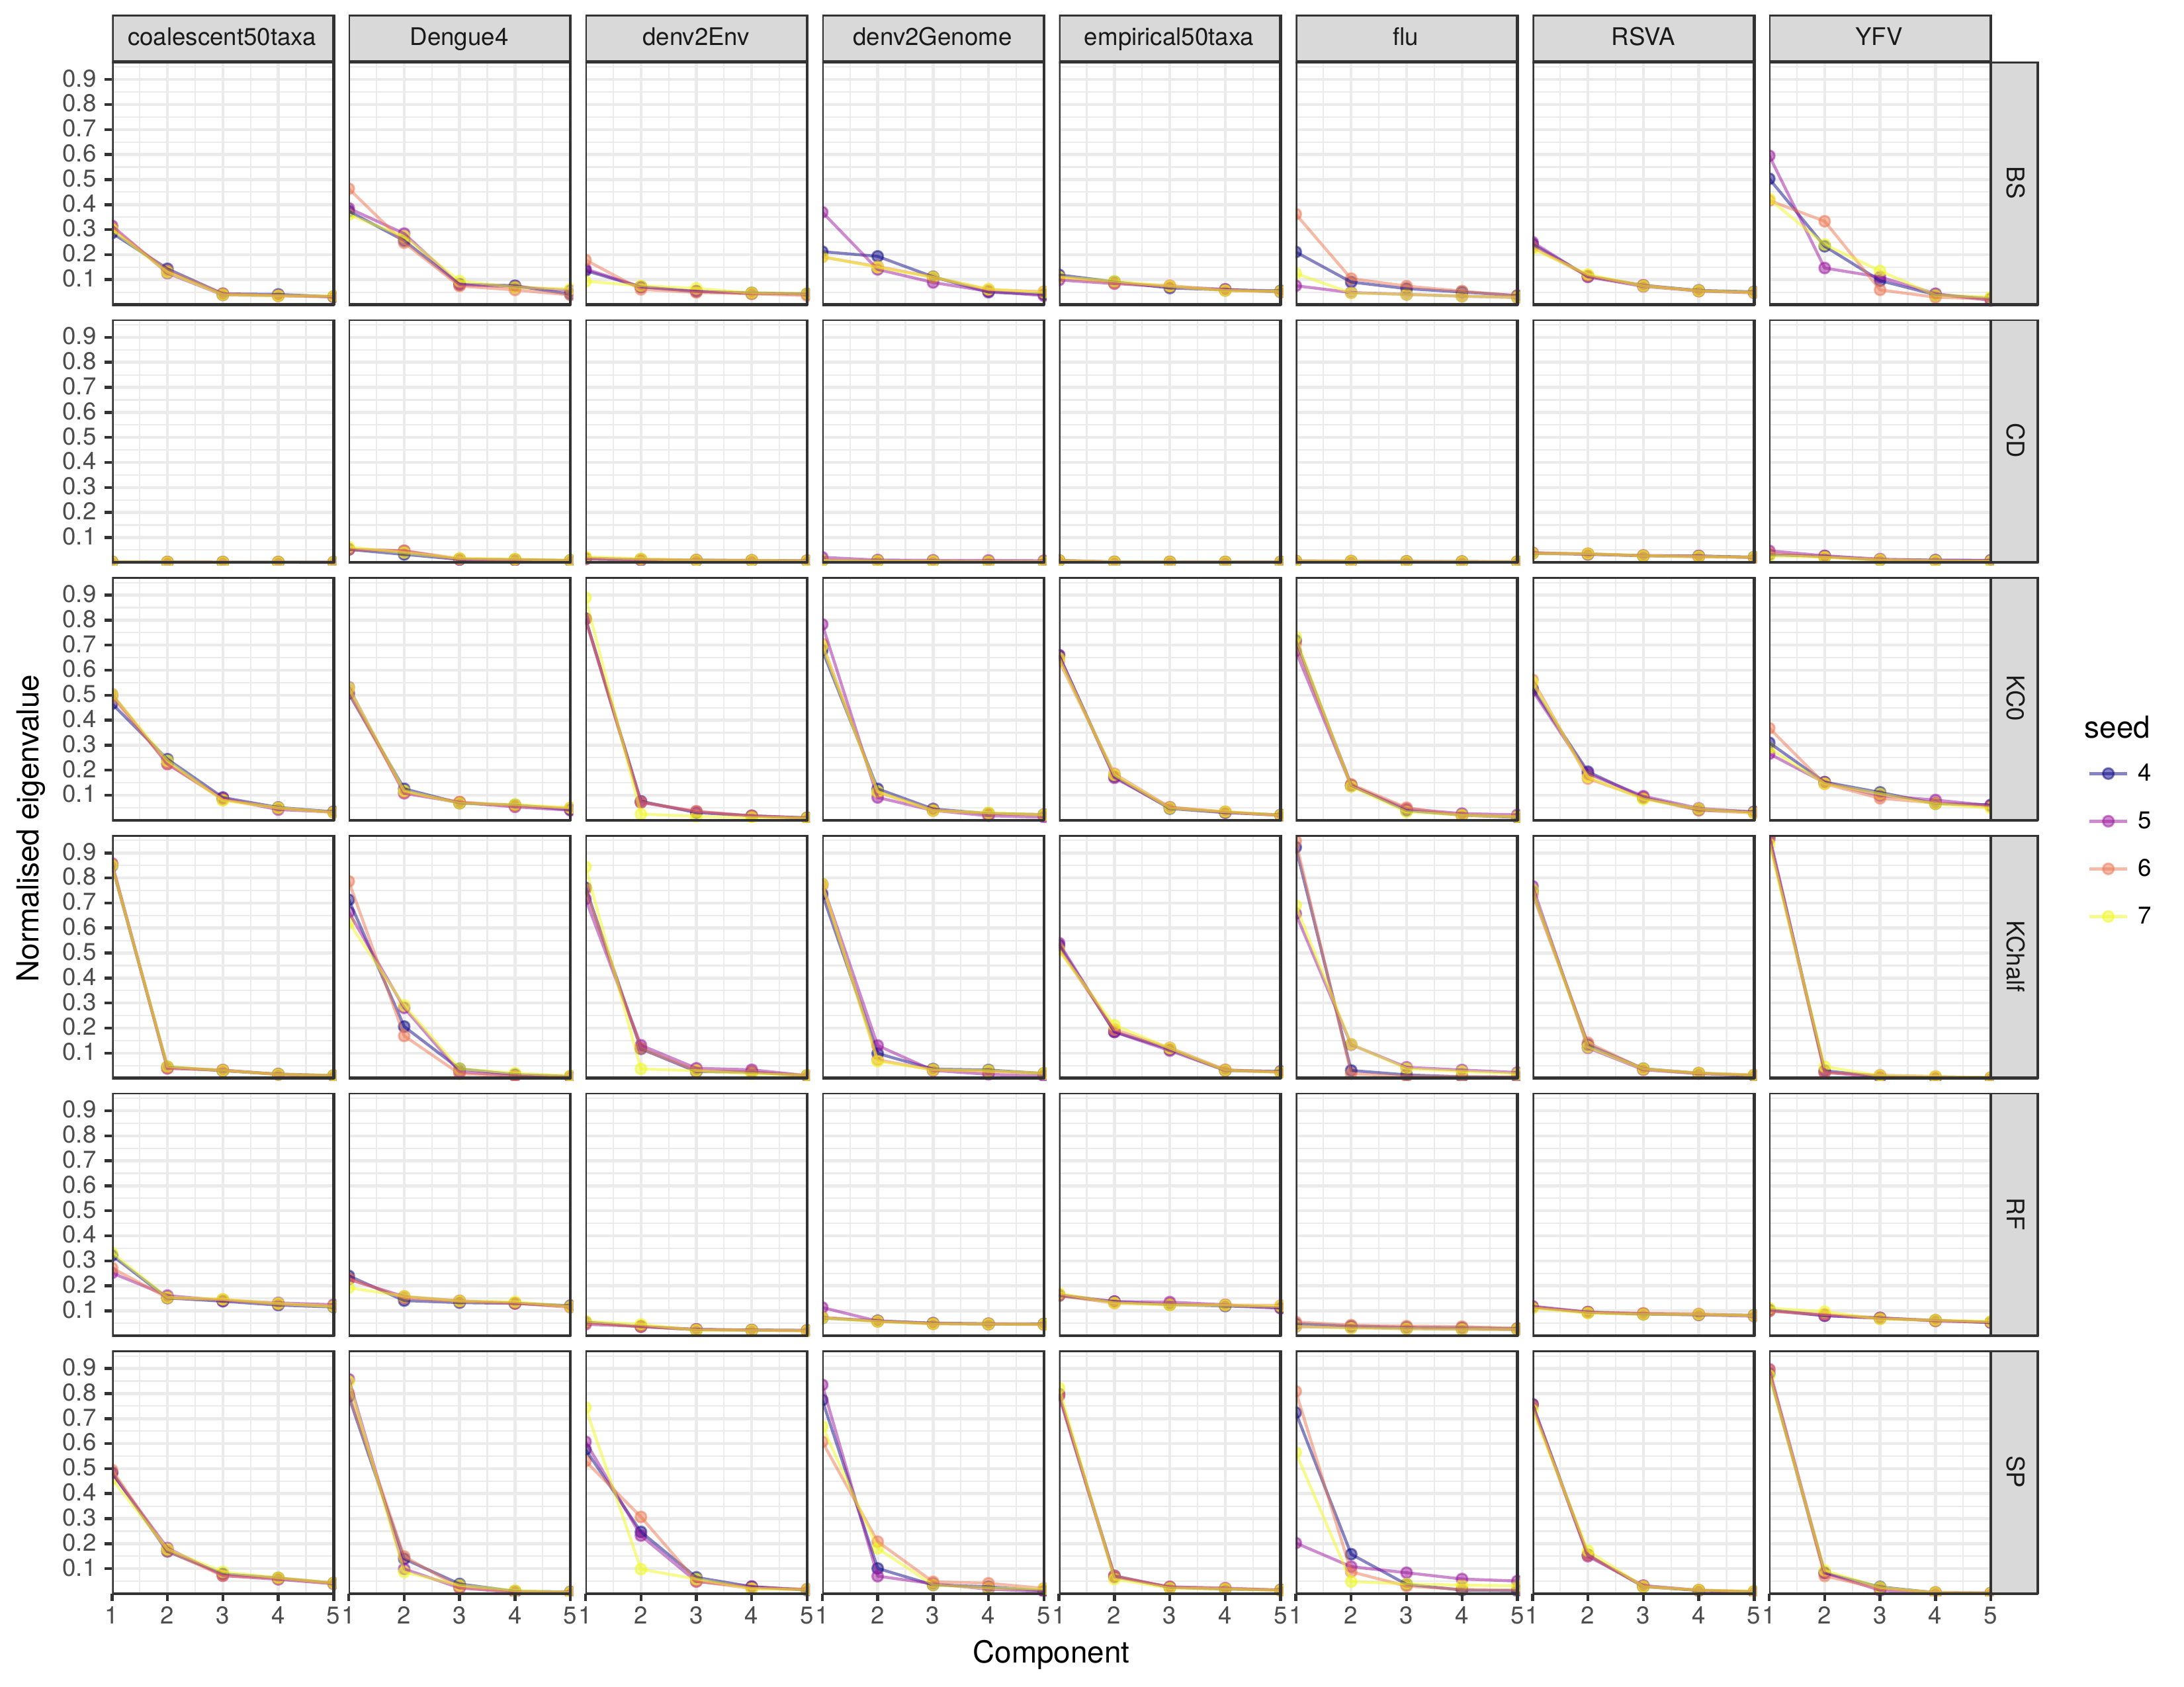
\includegraphics[scale=0.55]{\dir/figs/scree_plots_mds.png} 
\end{center}
 \caption[Scaled eigen values of phylogenetic space MDS.]{\textbf{Scaled eigen values of phylogenetic space MDS.}
 Vertical tiling shows the data set and horizontal ones show the phylogenetic metric used.
 Colours relate to the seed used in the pseudo random number generator, ensuring each run starts from the same point. 
 ``Elbow-shaped'' plots indicate fewer components are needed to capture the variation in the data.
 }
 \label{fig:screeplots}
\end{figure}

\subsection{Typical set for phylogenies}
\label{sec:typical}

One question one might ask is, what does phylogenetic space look like when we know the right answer?
In this section I offer a first stab at this question by analysing a simulated data example with $50$ taxa (Section~\ref{sec:simudata}).
I present trace plots of the distance to the true tree and MDS projections of the posterior distributions under various metrics, marking the maximum clade credibility (MCC) trees obtained from each run of each operator mix and the true tree used to generate the data.
In Figure~\ref{fig:mds_50taxa_RF}, I show the MDS projection of the RF distances between trees sampled using three MCMC schemes (``operator mixes'' or MCMC schemes, see Chapter 2), under two generating models: a tree drawn from the coalescent and an empirical tree extracted from a real-world data sets.
We can see that as the amount of data increases, the posteriors become more concentrated around the true value, as do the MCC trees, as expected.
While this behaviour is present for both true trees (coalescent or empirical), the posteriors for the coalescent generating tree seem to be more variable.

\begin{figure}[!ht]
\begin{center}
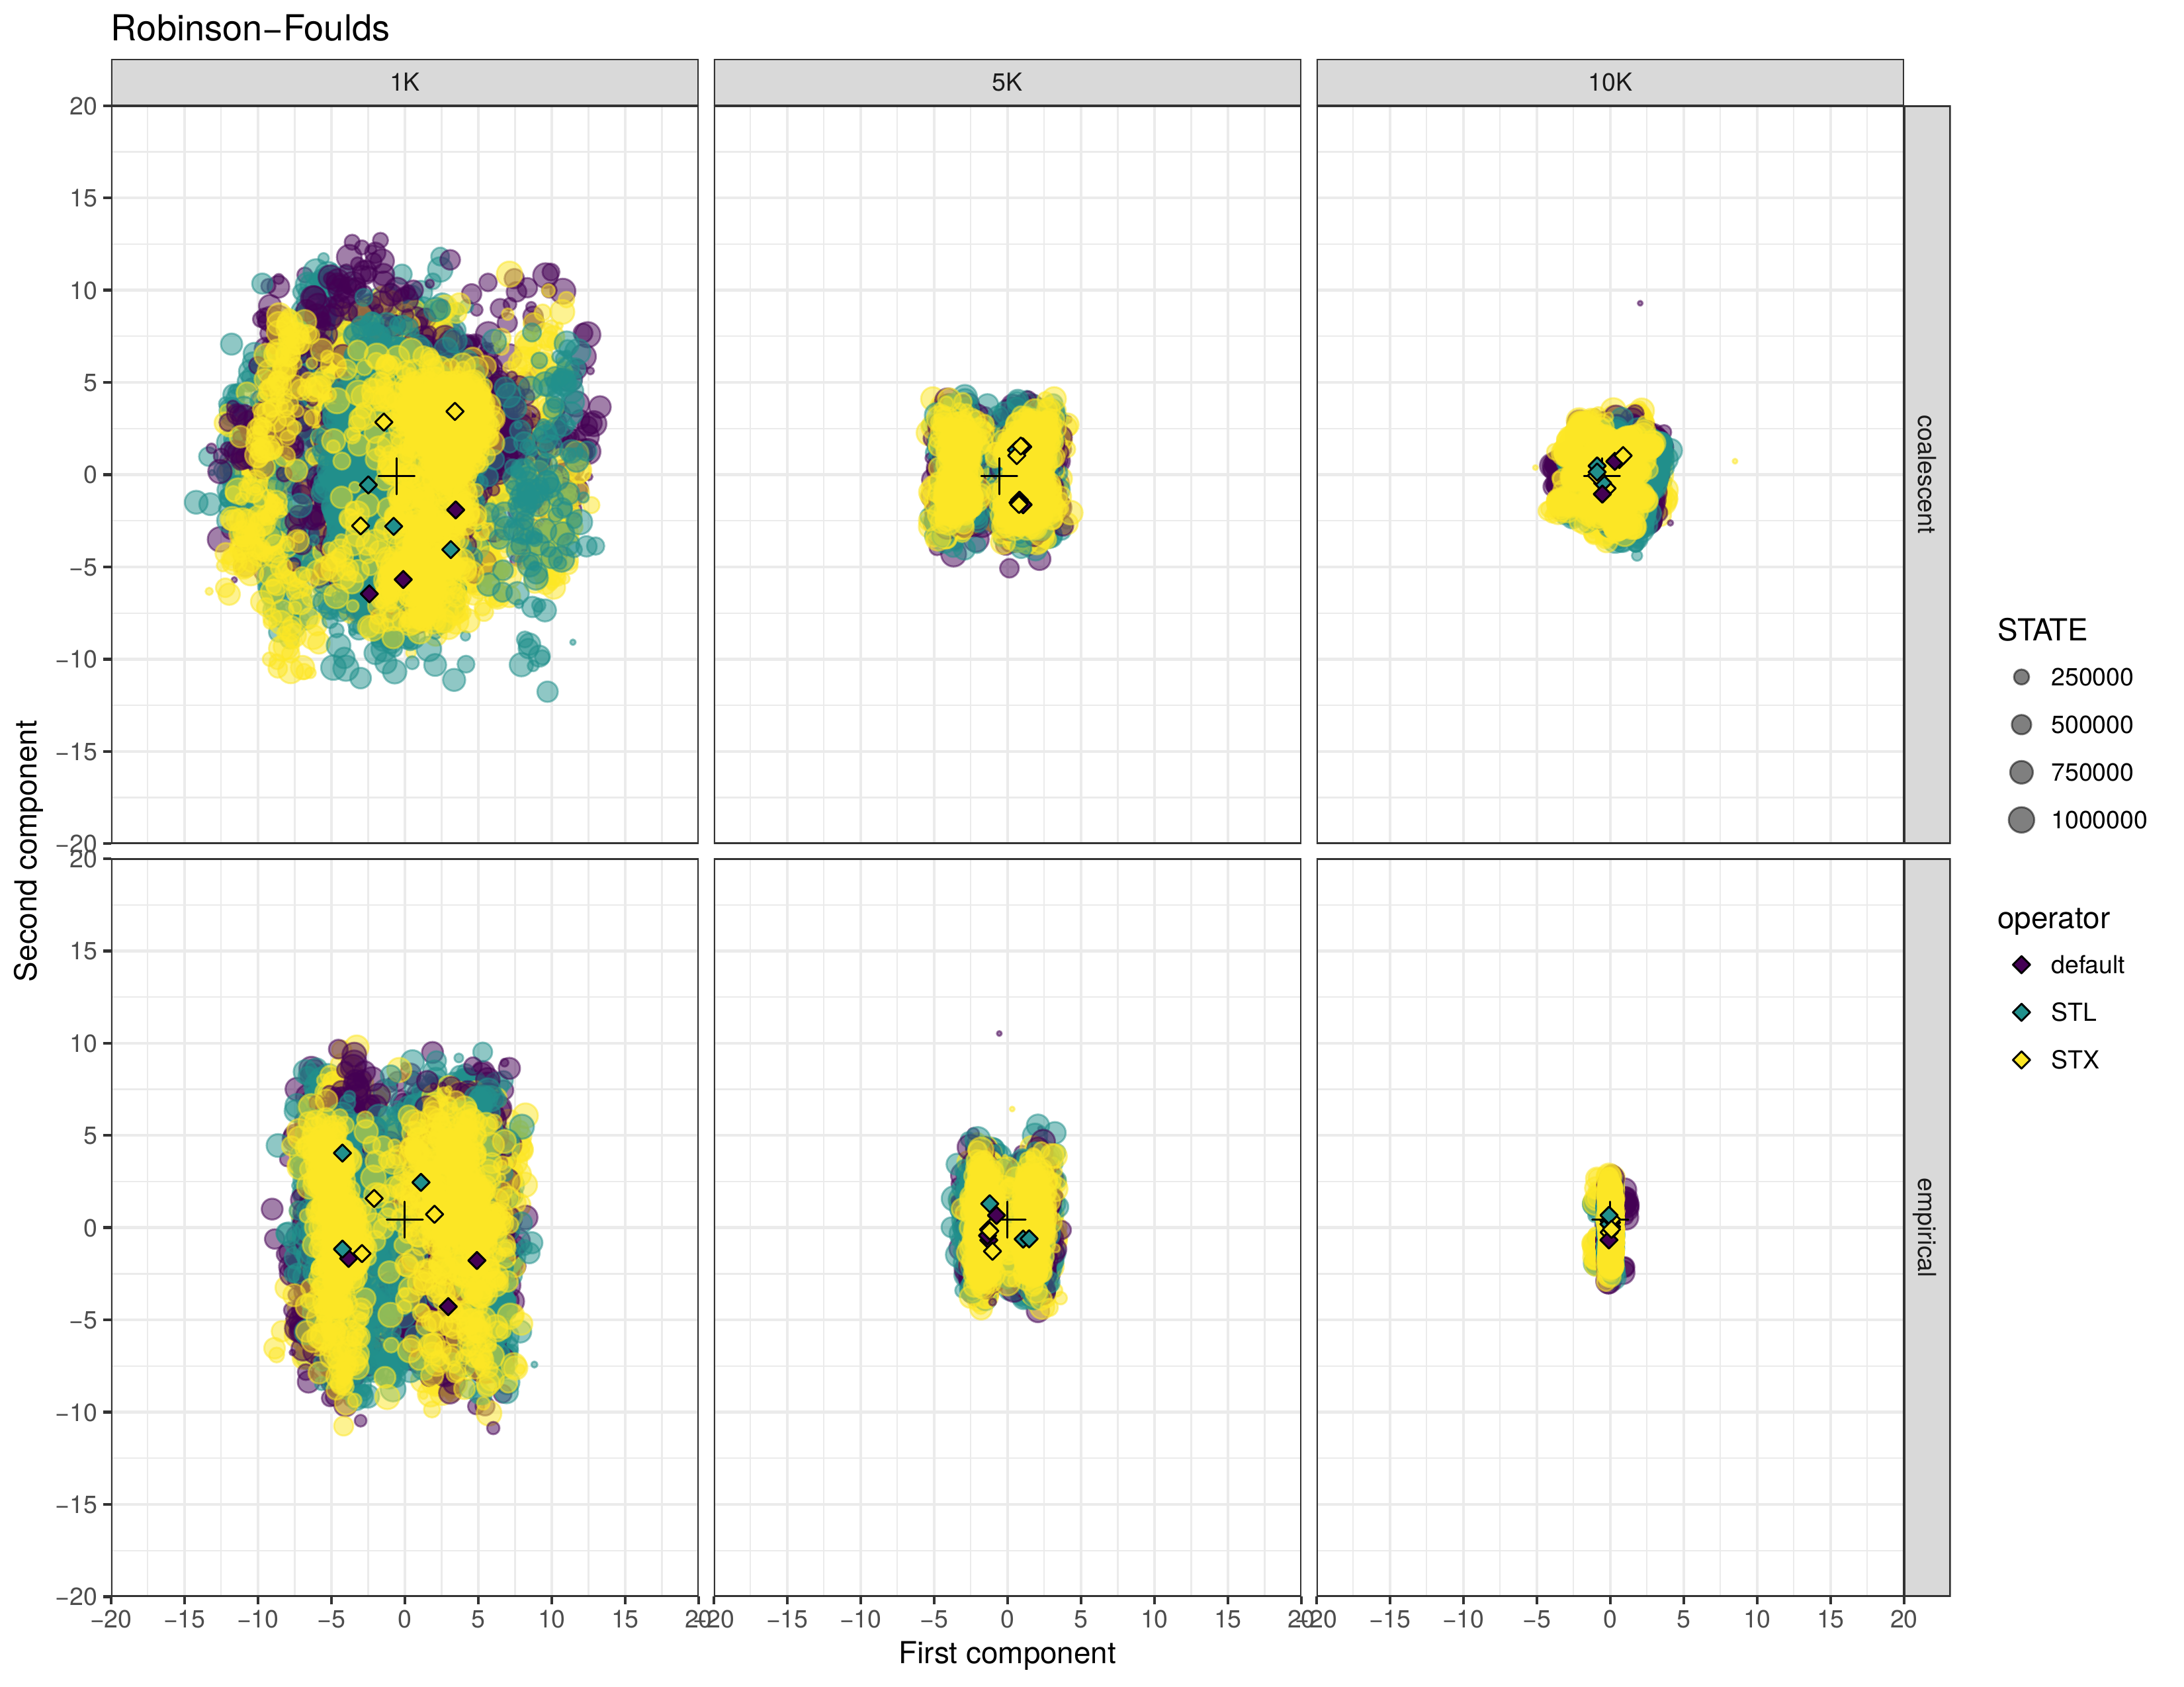
\includegraphics[scale=0.5]{\dir/figs/mds_50taxa_RF.png} 
\end{center}
 \caption[MDS projections for the simulated 50 taxa data set (Robinson-Foulds distances).]{\textbf{MDS projections for the simulated 50 taxa data set (Robinson-Foulds distances).}
  I show three replicates per operator, 1000 trees in each replicate, computing the RF distance between all pairs of trees.
  The cross marks the true tree used to simulate the data.
 Colours pertain to the combination of MCMC transition kernels used and solid diamonds mark the maximum clade credibility (MCC) trees obtained from each run.
 Horizontal panels show the true tree: either drawn from the coalescent or extracted from a real world data set (``empirical'').
 Vertical panels show the number of sites in the simulated alignment (1000, 5000 or 10 000).
 Please see Section~\ref{sec:simudata} for more details.
 }
 \label{fig:mds_50taxa_RF}
\end{figure}

Under the KC metric with $\lambda = 0$ (Figure~\ref{fig:mds_50taxa_KC0}), we observe a very similar pattern, but for this data set this representation more clearly shows the topological modes and how the MCC trees approach the correct mode (that contains the true tree) as the amount of data grows (rightmost bottom panel) .
Also from this panel we see that the posterior for the empirical generating tree also show markedly separate modes when compared to coalescent generating tree.
Since this representation captures only topological features, I claim that the differences must be due to the implicit interaction between branch length distribution and topology. 
An interesting observation is that the default operators sometimes lead to samples outside the typical set even when the chain is supposed to have converged to the target (rightmost top panel).
\begin{figure}[!ht]
\begin{center}
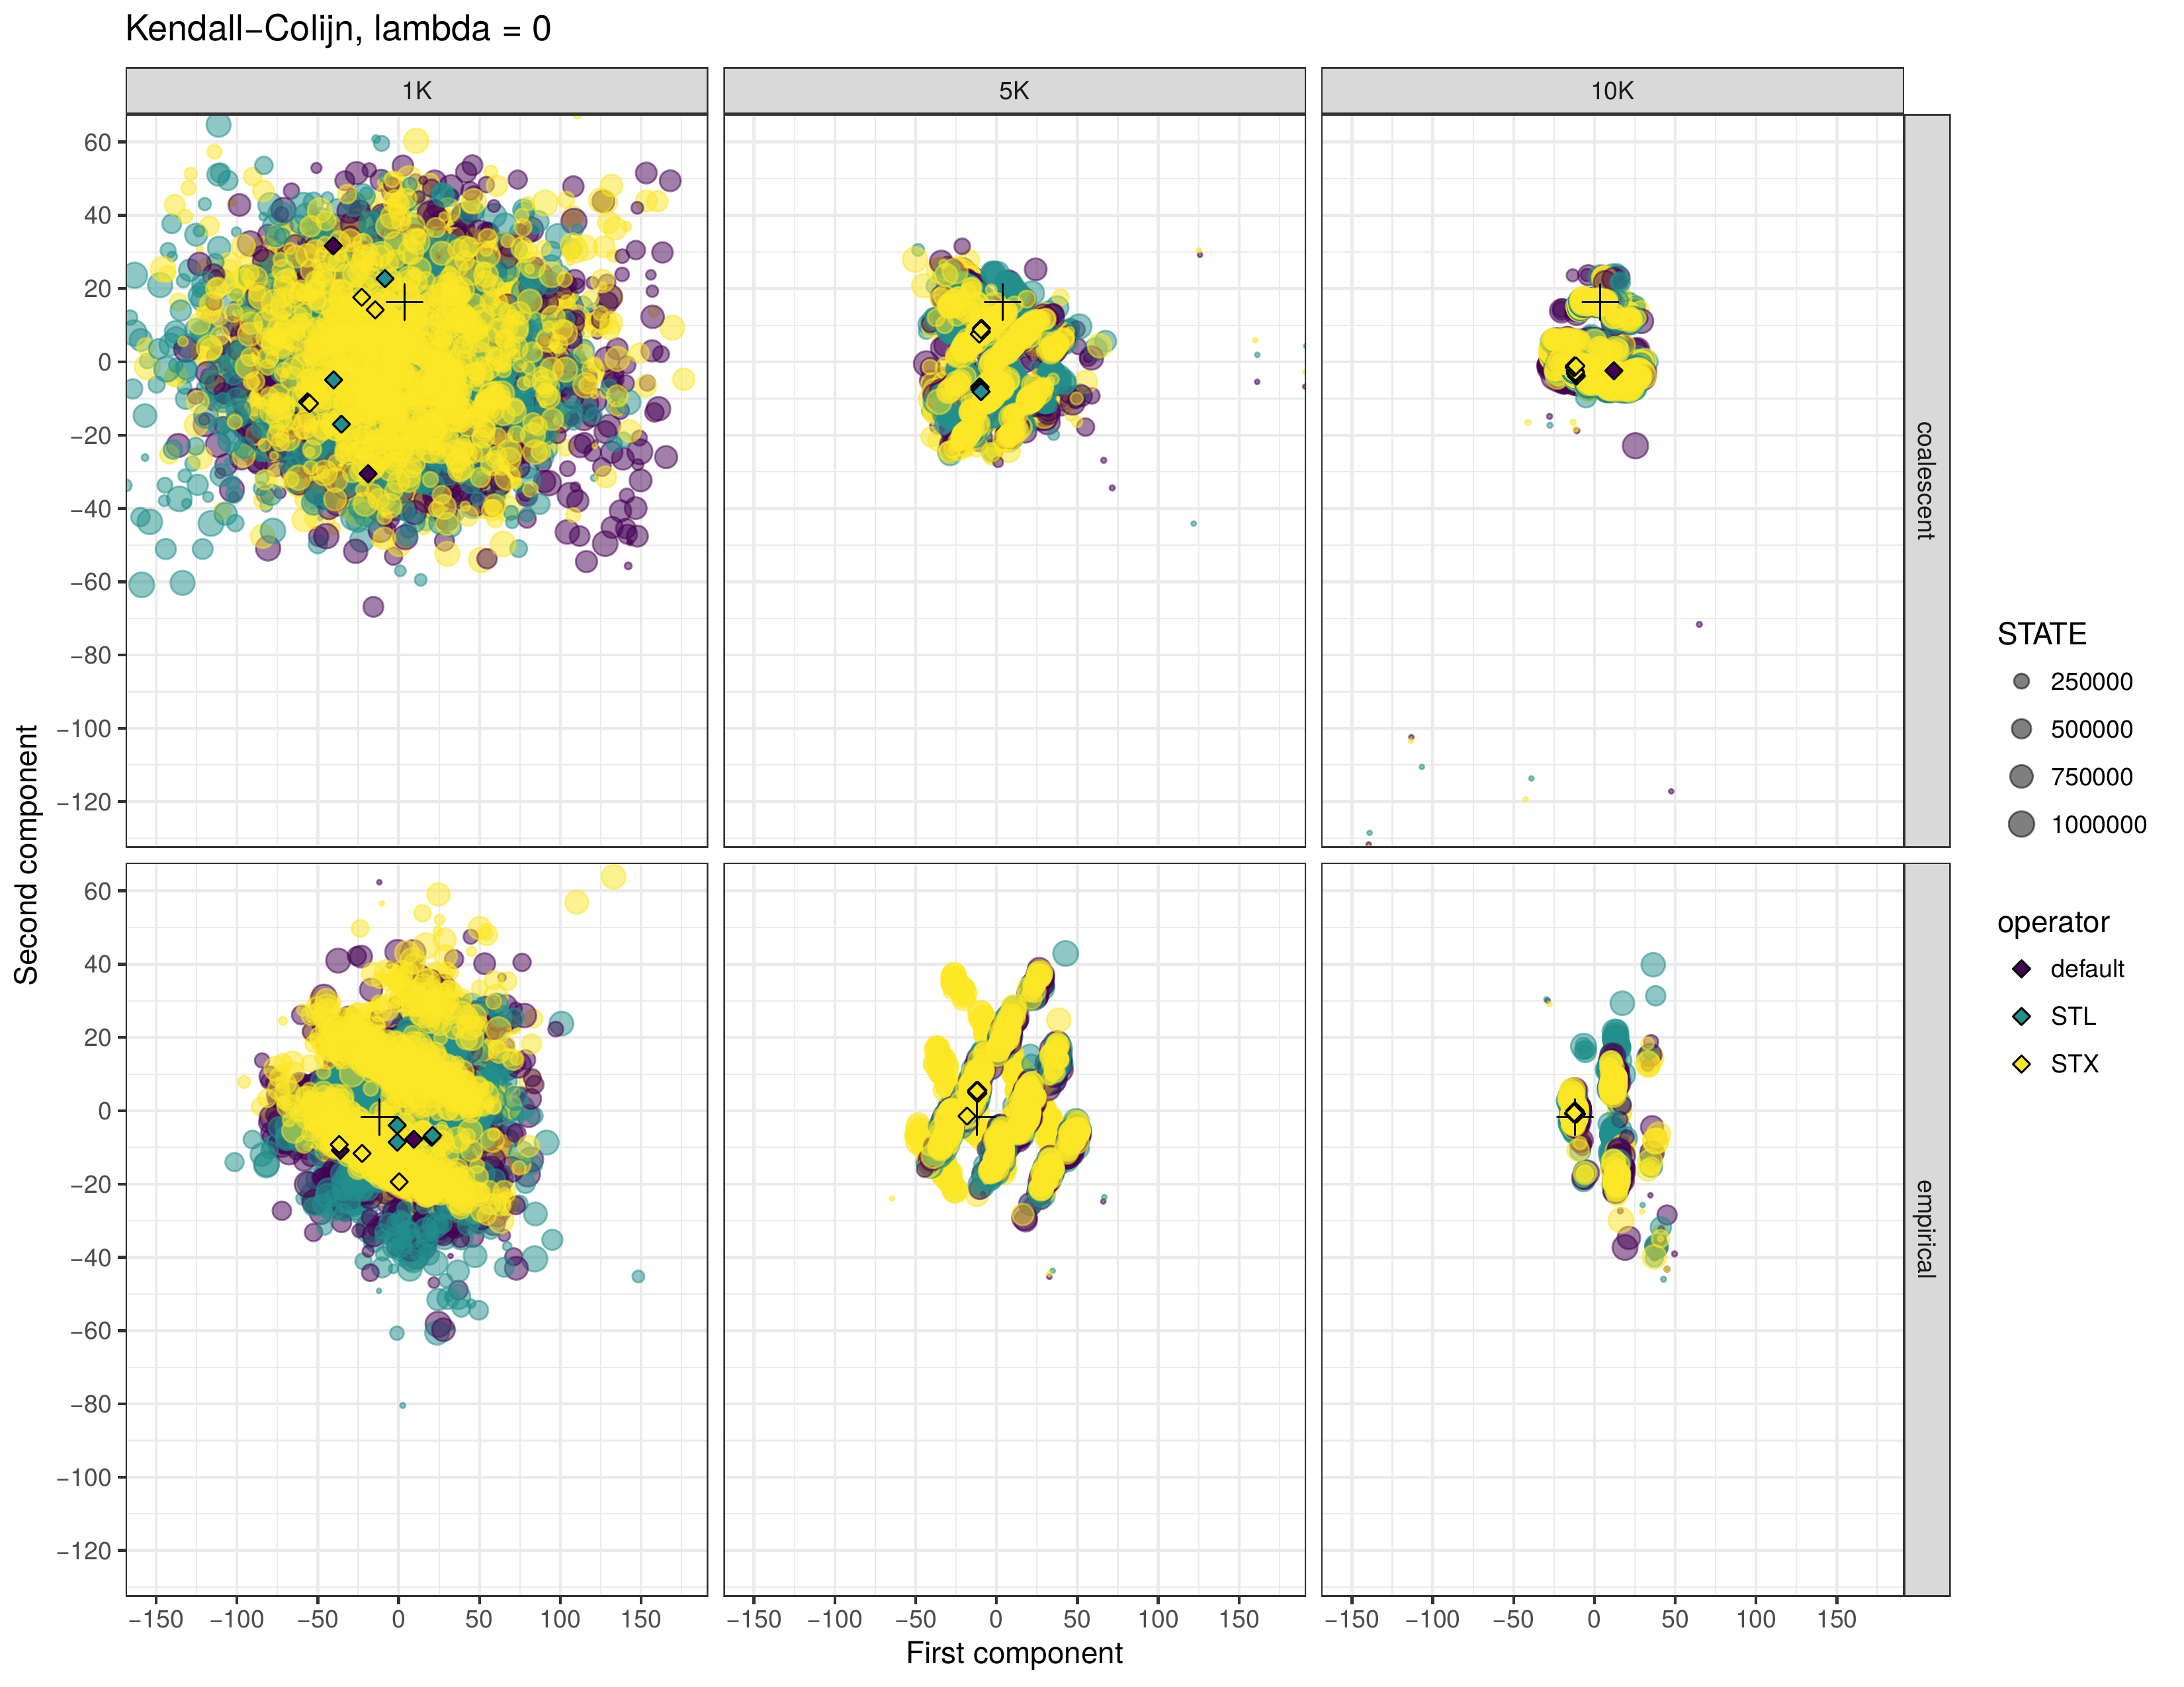
\includegraphics[scale=0.5]{\dir/figs/mds_50taxa_KC0.png} 
\end{center}
 \caption[MDS projections for the simulated 50 taxa data set (Kendall-Colijn distances).]{\textbf{MDS projections for the simulated 50 taxa data set (Kendall-Colijn distances).}
  I show three replicates per operator, 1000 trees in each replicate, computing the KC distance between all pairs of trees.
 The cross marks the true tree used to simulate the data.
 Colours pertain to the combination of MCMC transition kernels used and solid diamonds mark the maximum clade credibility (MCC) trees obtained from each run.
 Horizontal panels show the true tree: either drawn from the coalescent or extracted from a real world data set (``empirical'').
 Vertical panels show the number of sites in the simulated alignment (1000, 5000 or 10 000).
 See Figure~\ref{fig:mds_50taxa_RF} for a projection of the same trees under the RF metric.
 }
\label{fig:mds_50taxa_KC0}
\end{figure}

In keeping with the results in Section~\ref{sec:representation}, the Steel-Penny metric leads to MDS projections that appear smoother (Figure~\ref{fig:mds_50taxa_SP}).
Also noteworthy is the amount of samples outside the typical set observed for the default kernels (small purple dots). 
Taken together with Figures~\ref{fig:mds_50taxa_RF} and~\ref{fig:mds_50taxa_KC0}, these results show progressive concentration of the posterior around the true value with alignment size (number of sites), even if posteriors for the empirical generating tree seem less smooth and harder to sample from.
\begin{figure}[!ht]
\begin{center}
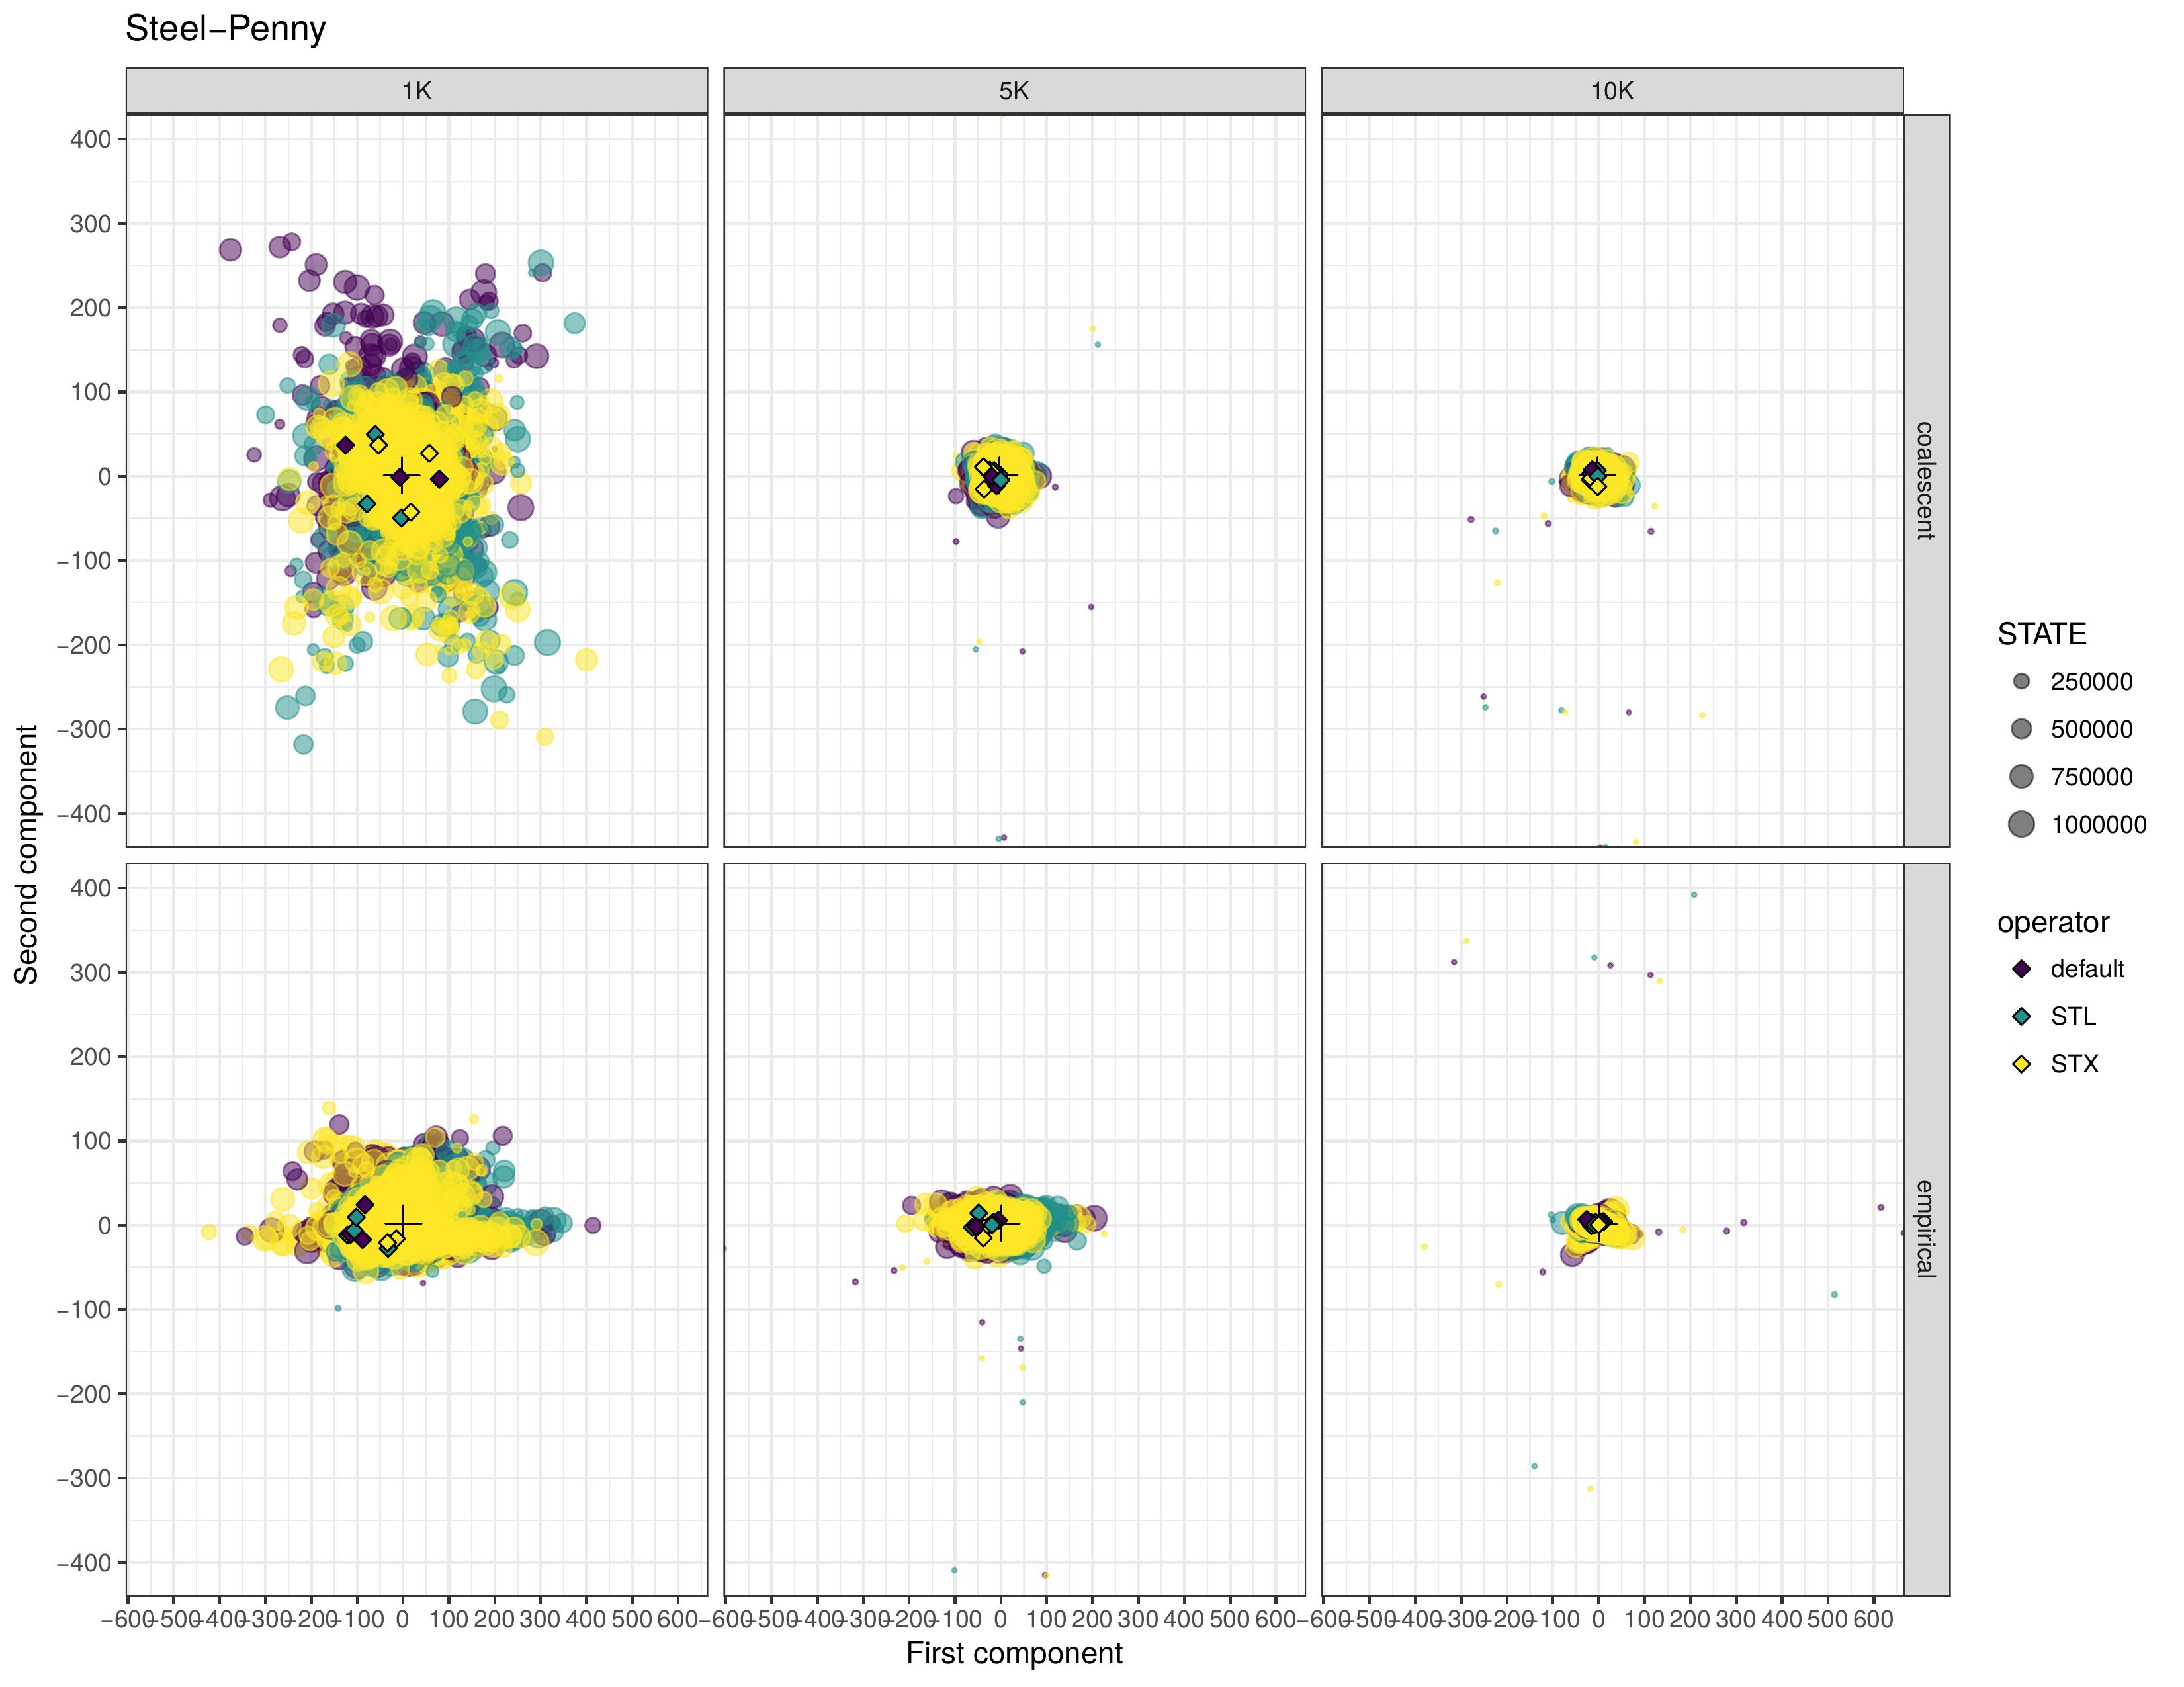
\includegraphics[scale=0.5]{\dir/figs/mds_50taxa_SP.png} 
\end{center}
 \caption[MDS projections for the simulated 50 taxa data set (Steel-Penny distances).]{\textbf{MDS projections for the simulated 50 taxa data set (Steel-Penny distances).}
 I show three replicates per operator, 1000 trees in each replicate, computing the SP distance between all pairs of trees.
 Colours pertain to the combination of MCMC transition kernels used and solid diamonds mark the maximum clade credibility (MCC) trees obtained from each run.
 Horizontal panels show the true tree: either drawn from the coalescent or extracted from a real world data set (``empirical'').
 Vertical panels show the number of sites in the simulated alignment (1000, 5000 or 10 000).
 See Figure~\ref{fig:mds_50taxa_RF} for a projection of the same trees under the RF metric.
 }
\label{fig:mds_50taxa_SP}
\end{figure}

When we know the true tree, we can also study phylogenetic space and its exploration \textit{via} MCMC by computing the distance to the true tree and tracking how the distance changes through the chains as well as the resulting distributions.
In this simulated example we can exploit the fact that we know the true tree to the visualisation/analysis problem to essentially one dimension.
We can look at the resulting distributions as if they were univariate targets, which in turn facilitates visualisation and intuition-building, in addition to making it possible to apply a plethora of statistical methods developed for the analysis of univariate distributions.
While in practice we do not know the true tree, these simulations are useful for understanding the behaviour of transition kernels and MCMC in general. 

In Figure~\ref{fig:topo_distances_50taxa} I show the results of this analysis for the 50 taxa simulated example discussed above, for topological metrics (RF and KC)  in order to show the combinatorial (discrete) multimodality of phylogenetic space.
The first pattern to notice is that the number and location of peaks changes as the amount of information increases (colours).
Secondly, I highlight how running the chains for longer leads to better defined peaks, even though for this simple example\footnote{Recall that in this example the parameters are inferred under the generating model,\textit{i.e.} there is no model misspecification.} 10 million iterations seem to be adequate to find and explore all of the detected modes.
Also noticeable is how diffuse the target for the coalescent tree is for a small alignment size (one thousand sites) under the KC metric (Figure~\ref{fig:topo_distances_50taxa}, panel D).
While the target intermediate alignment shows bimodality, the target for 10 thousand sites shows three modes, one much bigger than the other two.
Overall the empirical generating tree leads to more complex posteriors, specially for the intermediate alignment size (panel B, red curve).

\begin{figure}[!ht]
\begin{center}
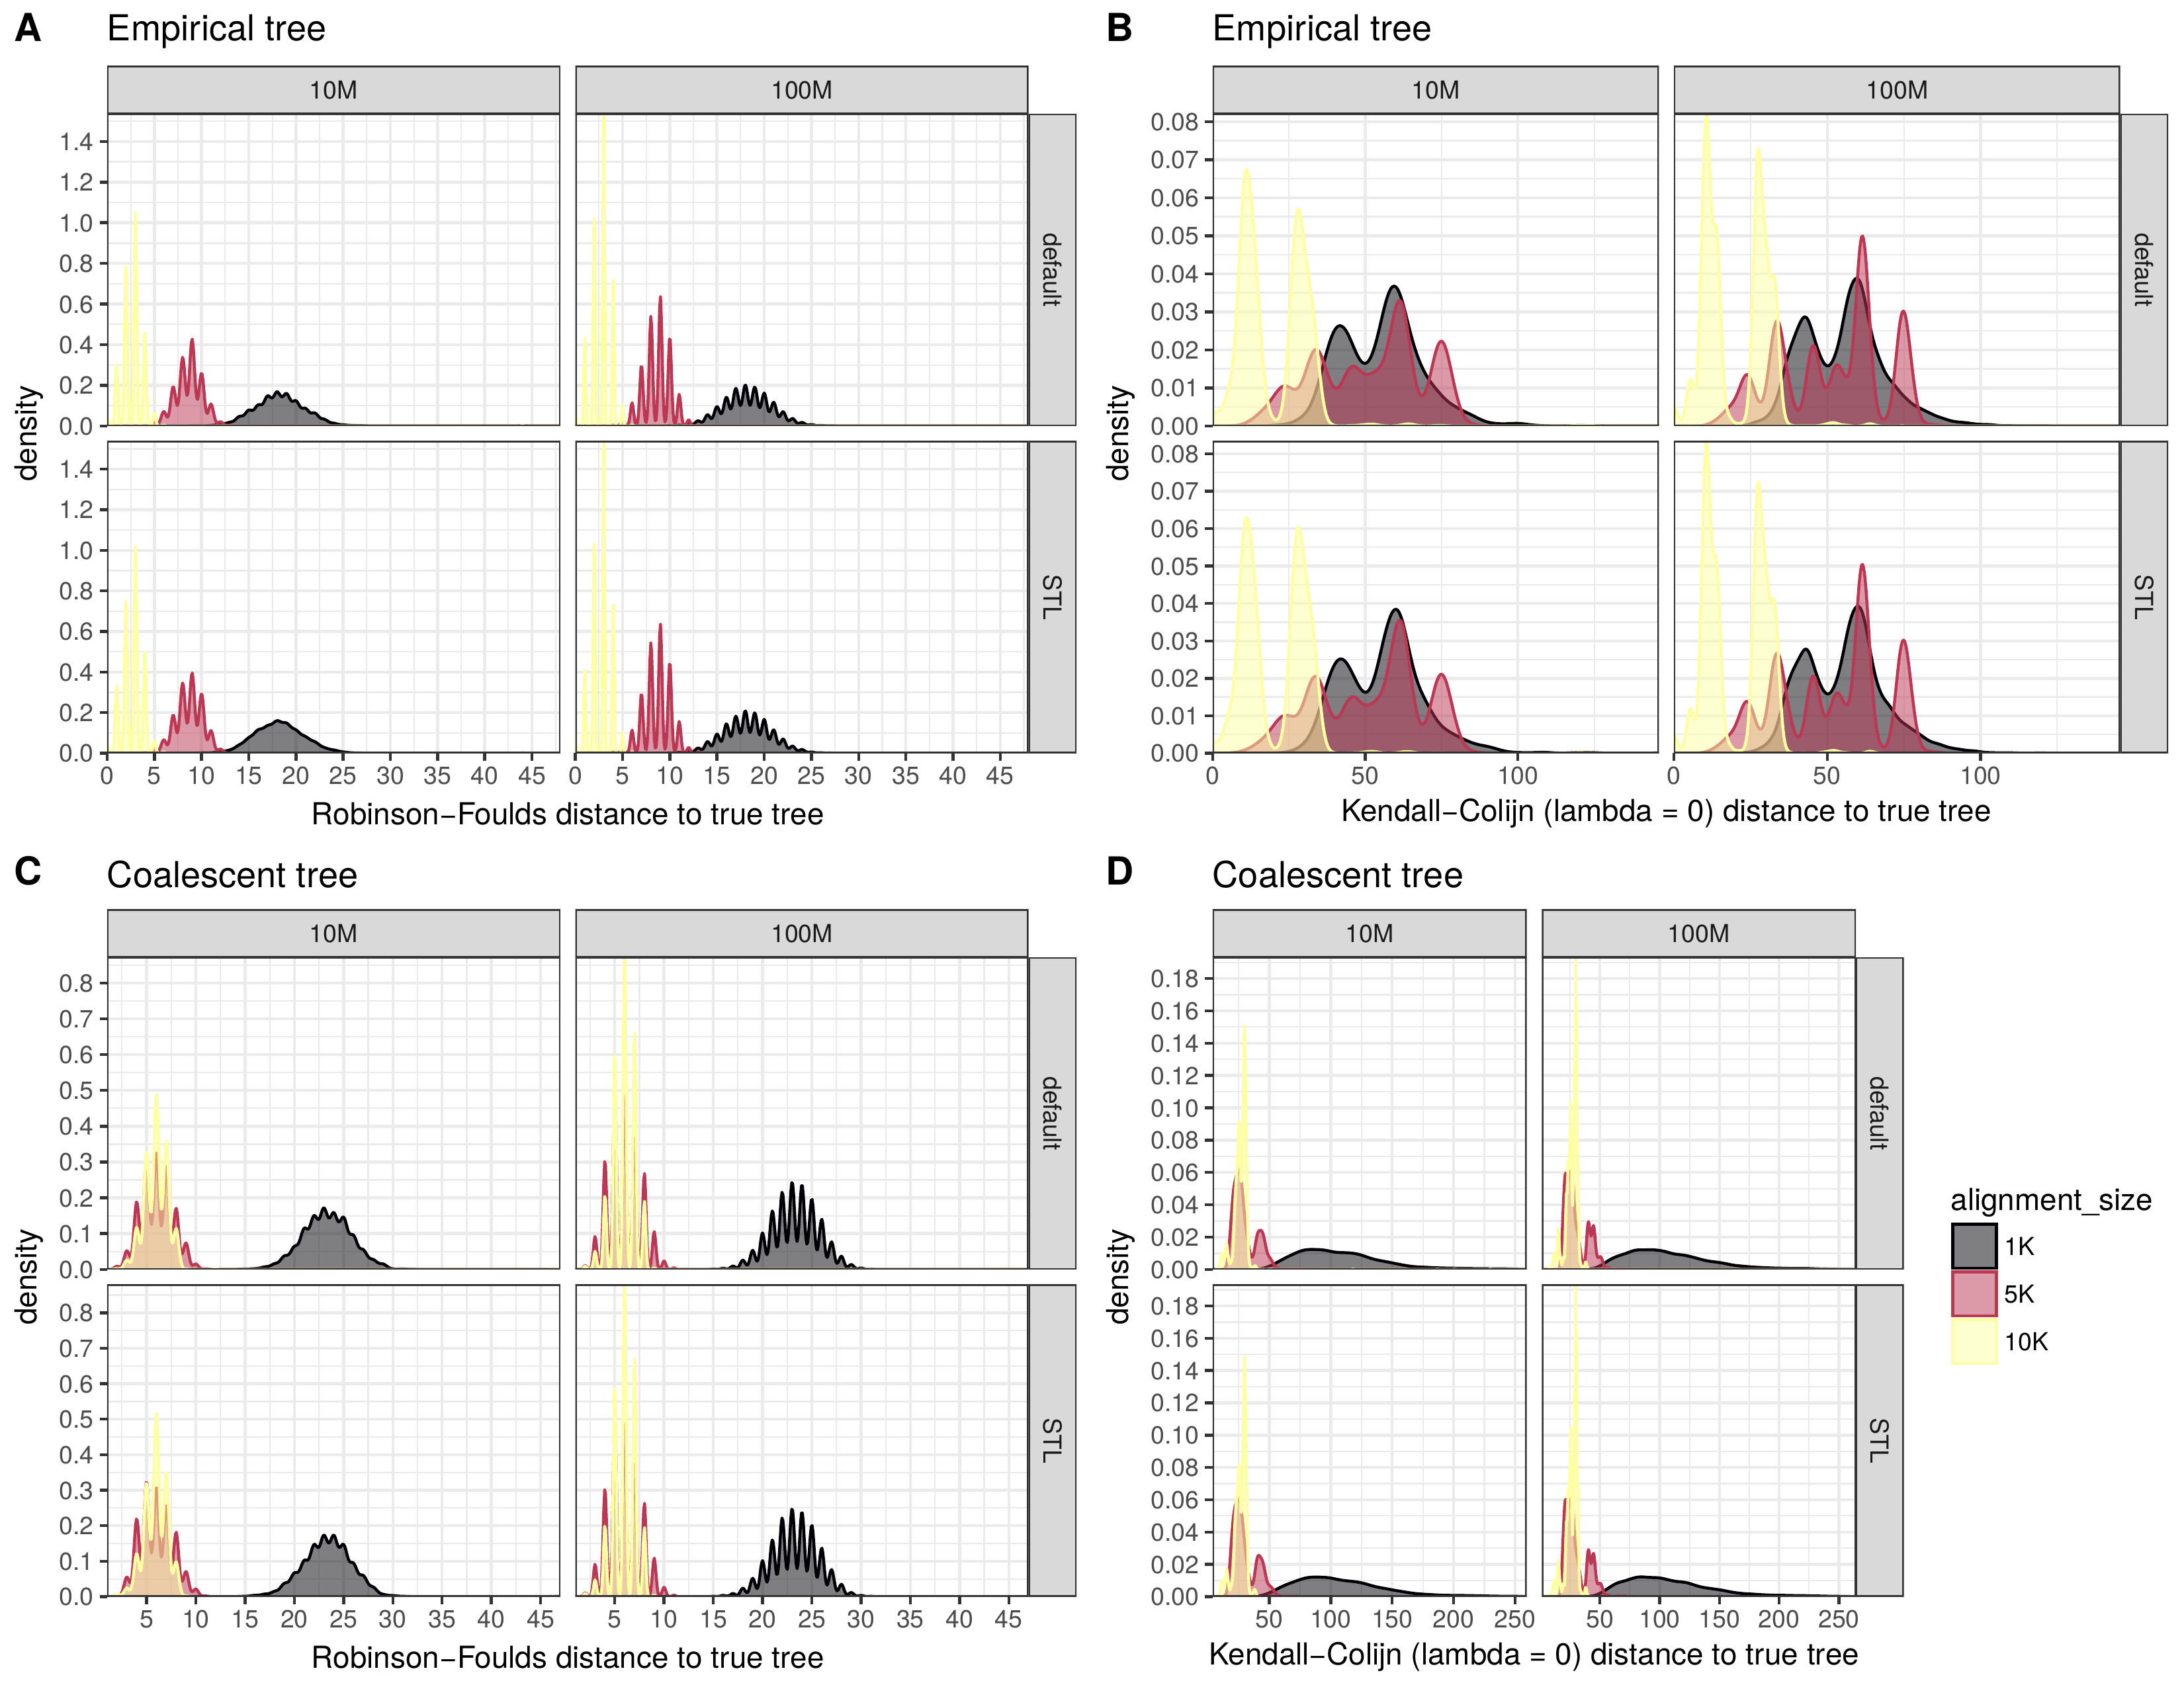
\includegraphics[scale=0.55]{\dir/figs/topo_distance_to_true_tree_50taxa.png} 
\end{center}
 \caption[Characterisation of topological modes for a simulated example (50 taxa).]{\textbf{Characterisation of topological modes for a simulated example (50 taxa).}
  I ran chains of 10 and 100 million iterations for three alignment sizes and two generating trees (see Chapter 2 for more details).
 Panels A and C show the Robinson-Foulds~\citep{Robinson1981} distance to the tree, while panels B and D show the Kendall-Colijn~\citep{Kendall2016} distance, with $\lambda =0$ (topology only). 
 Vertical panels show the chain length used, while horizontal panels display results obtained with different sets of transition kernels.
 }
 \label{fig:topo_distances_50taxa}
\end{figure}

When we turn attention to metrics that incorporate branch length information (Figure~\ref{fig:cont_distances_50taxa}), another interesting pattern emerges: while the SP metric leads to smooth targets, the KC metric shows distinct multimodality for the empirical generating tree.
It is difficult to say whether these observed differences are due to some underlying fundamental distinction or just an artefact specific to the two trees used -- there were no replicates at generating tree level of the experiment.
This result calls for further investigation into the inherent differences between empirical trees,~\textit{i.e.}, trees that are estimated from data encountered in practice, and their coalescent counterparts (see Section~\ref{sec:conclusion}).

\begin{figure}[!ht]
\begin{center}
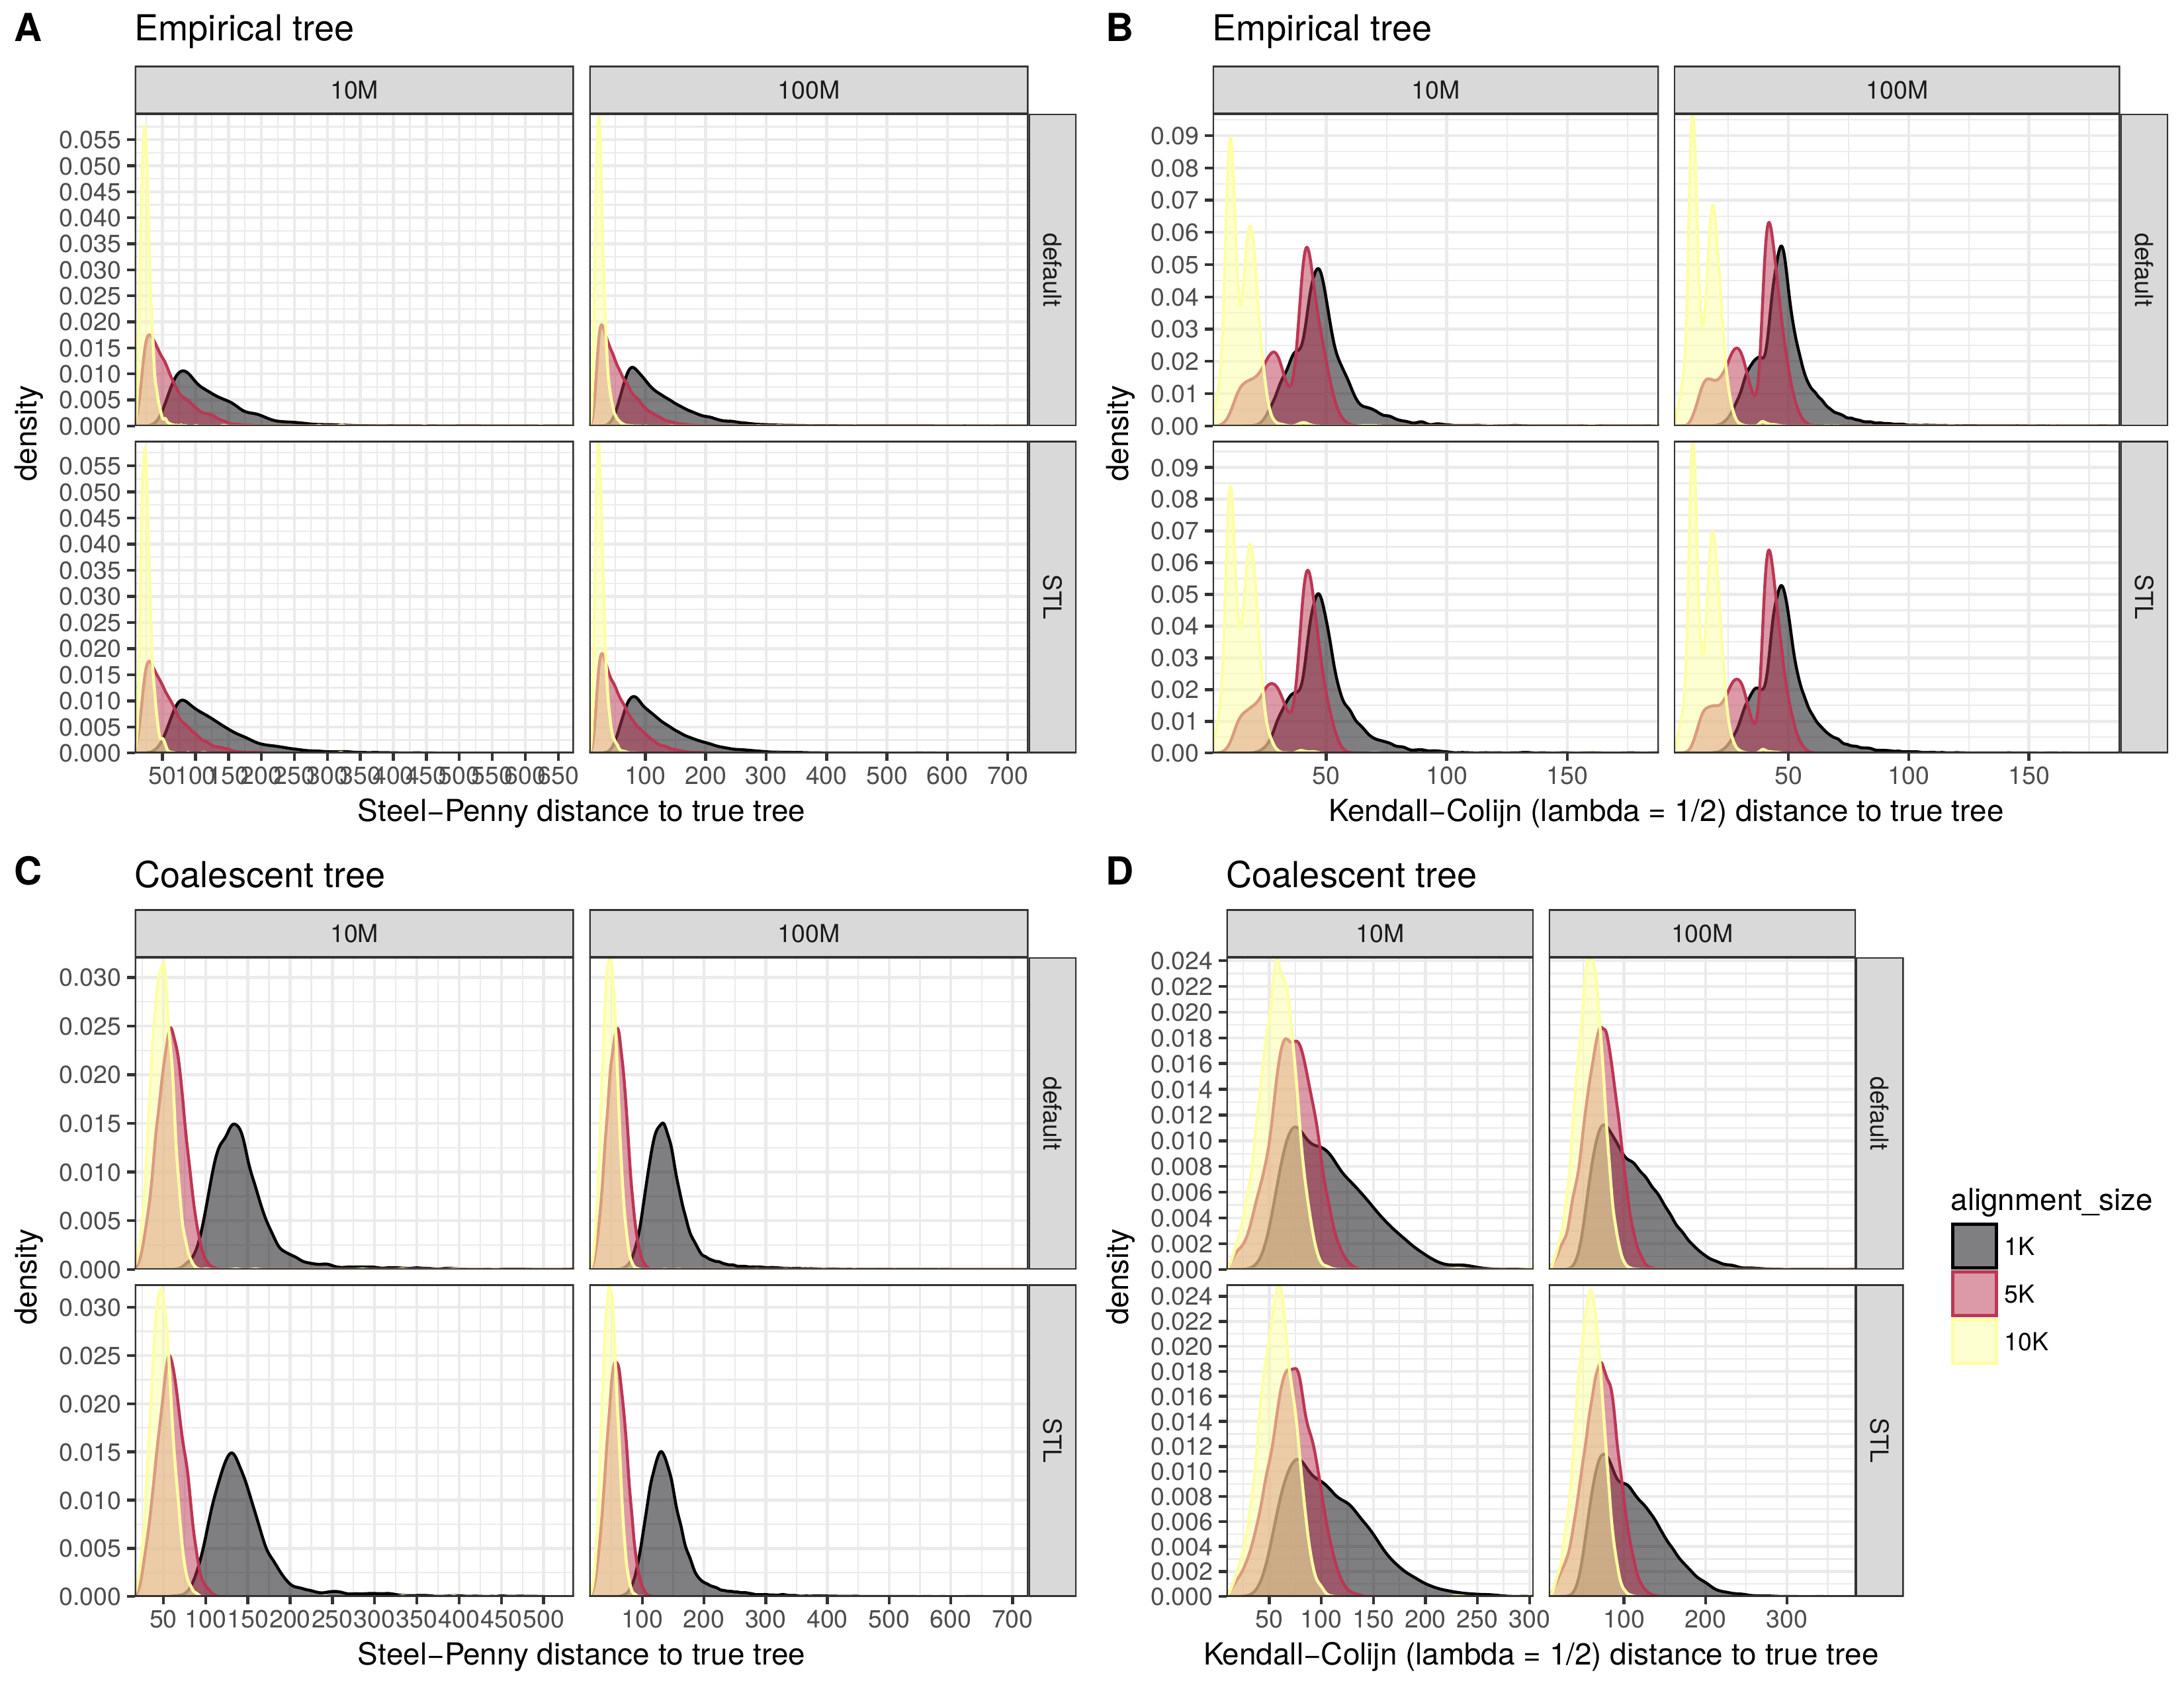
\includegraphics[scale=0.55]{\dir/figs/cont_distance_to_true_tree_50taxa.png} 
\end{center}
 \caption[Characterisation of continuous phylogenetic space for a simulated example (50 taxa).]{\textbf{Characterisation of continuous phylogenetic space for a simulated example (50 taxa).}
  I ran chains of 10 and 100 million iterations for three alignment sizes and two generating trees (see Chapter 2 for more details).
 Panels A and C show the Steel-Penny~\citep{Steel1993} distance to the tree, while panels B and D show the Kendall-Colijn~\citep{Kendall2016} distance with $\lambda = 1/2$,  which accounts for both topology and branch lengths. 
 Vertical panels show the chain length used, while horizontal panels display results obtained with different sets of transition kernels.
 }
 \label{fig:cont_distances_50taxa}
\end{figure}
Figures~\ref{fig:topo_distances_50taxa} and~\ref{fig:cont_distances_50taxa} also illustrate how casting the phylogeny sampling problem as a univariate sampling problem allows one to more clearly compare MCMC strategies.
Under both representations it is clear that \verb|SubTreeLeap| leads to virtually identical samples to those obtained with the default set of transition kernels, increasing confidence in the correctness of its implementation (see Chapter 2, Section~\ref{sec:correctness}). 
Moreover, it also seems to find and sample from all the detected modes, even for complex distributions such as those in panel B of Figure~\ref{fig:topo_distances_50taxa}.

While reducing the problem to a univariate quantity is an attractive idea (see, e.g. ``Method 1'' in ~\cite{Lanfear2016}), it is generally not possible in practice since we do not know the true tree and the choice of focal tree is arbitrary.
In the context of the development of phylogenetic transition kernels, however, I believe this method can be useful in constructing univariate representations of the target distribution, and thus allow us to leverage a vast body of theory available for assessing performance and correctness.
See Section~\ref{sec:mcmc_efficiency} in Chapter 2 for more details on how this  framework can be applied to evaluate MCMC mixing.

\section{Final remarks}
\label{sec:conclusion}

In this chapter I have sought to supplement the toolbox of diagnostic measures for MCMC in phylogenetic space with a few new tools and other tools seldom used in the field.
I by no means claim to have provided the first workflow of this kind, however.
Previous studies such as~\cite{Hillis2005},~\cite{Lakner2008},~\cite{Nylander2008} and~\cite{Warren2017} have touched on many of the aspects tackled here.
The research reported here is an attempt at combining previous approaches with new metrics while overcoming some of the technical hurdles imposed by large time-calibrated phylogenies impose.

The results for the ``poor'' runs (Table~\ref{tab:continuous_results}) are not surprising since the chain was deliberately designed to mix poorly in phylogenetic space.
A perhaps more subtle point to be made, however, is that since parameters vary regarding their inherent dependence on the phylogeny, computing global convergence metrics including all parameters might mask convergence problems.
This could be easily fixed by separating parameters into blocks when assessing convergence; more phylogeny-dependent parameters could be paid special attention.
Of course it is not always easy to know how dependent on the underlying phylogeny a parameter is; further research is needed in order to determine whether/how to do parameter blocking.
The multivariate ESS results show that when accounting for correlations between parameters none of the tested MCMC schemes achieves a sufficient number of samples.
This is intimately linked with the common recommendation of declaring a run acceptable if it achieves marginal univariate ESSs larger than $200$ for all parameters.
The practical relevance of this rule is yet another topic for future research.

Regarding diagnostics specifically designed for phylogenies, the results in Table~\ref{tab:tree_results} suggest a lack of agreement between approximate ESSs computed using different tree metrics.
For instance, for the poorly mixing runs some ESSs computed using the clade difference (CD) and branch score (BS) are estimated as 1001, the maximal value, suggesting these metrics might not be reliable for discriminating between poorly mixing runs and adequately mixing ones.
These results are in tune with those presented in Section~\ref{sec:representation}, which show that MDS projections under some metrics fail to highlight differences between runs and thus indicate severe convergence problems. 
In contrast, Figure~\ref{fig:ESS_distance_true} in Chapter 2 shows that pseudo-ESS seems consistent between metrics -- the ranking between MCMC schemes is largely consistent --, at least in a setting where the focal tree is a summary tree from the tail end of three independent (long) golden runs.
Clade-based metrics seem to provide more discriminating tools, albeit the experimental setup does not allow definitive claims to be made.
As discussed in Section~\ref{sec:cladeSwitch}, correlation structure between clades complicates diagnostics based on marginal quantities, what seems to be corroborated by the fact that for the poorly mixing runs the mean univariate ESS for clade indicators was around $800$, which could mislead researchers into inferring acceptable mixing.

These inconsistencies seem to stem from the non-standard nature of phylogenetic space, which admits many representations without any one way of depicting the space being canonical.
The Billera-Holmes-Vogtman (BHV,~\cite{Billera2001}) cubical complex representation is a good candidate with good statistical properties, but distances are hard to compute, while others such as Kendall-Colijn metric are easier to compute but suffer from poor statistical and/or theoretical properties.
The KC metric for example suffers from an inherent scaling problem: when branch lengths and node indices are not commensurate, it is hard to calibrate $\lambda$ in order to obtain interpretable results.
A study in the same vein as~\cite{Kuhner2014} to compare the relative efficiency of tree metrics specifically for time-calibrated phylogenies is sorely needed.

The attentive reader will have noticed that while I mention and describe the BHV (geodesic) metric and associated space, none of my results include this metric.
This deserves explanation.
While conceptually I believe the BHV representation of phylogenetic space to be the most complete, enjoying many desirable properties (see~\cite{Billera2001},~\cite{StJohn2017} and~\cite{Dinh2016}), despite recent advances in the computation of the BHV metric~\citep{Owen2011} it still remains quite hard to apply to large time-trees.
Further programming work is needed to integrate the libraries provided by~\citep{Owen2011} into the framework described in this chapter.
In addition, if we are to approach phylogenetic inference as a statistical problem~\citep{Holland2013}, we need a representation that is statistically motivated so that results such as central limit theorems can be established.
Under such a representation, concepts such as effective sample sizes and typical sets are easier to interpret and analyse.
See Chapter 6 for a discussion of how BHV-based representations can be extended in that direction.

In summary, this chapter provides the following contributions/findings:
\begin{itemize}
 \item New analytical tools for a robust Bayesian phylogenetic analysis pipeline;
 \item For a given data set, some metrics can completely fail to indicate important differences between runs (compare Figures~\ref{fig:mds_ebov_RF},~\ref{fig:mds_ebov_KC} and~\ref{fig:mds_ebov_SP});
 \item Depending on the data set and metric, using just the first two components can be misleading (Figure~\ref{fig:screeplots});
 \item Approximate tree ESSs based on different metrics (distances) gave inconsistent results;
\end{itemize}

Several questions remain open however, which I intend to tackle in future research:

\begin{itemize}
 \item How exactly does sampling affect (the exploration of) phylogenetic space?
 The results in Section~\ref{sec:typical} suggest that, for a highly idealised situation (relatively few taxa, no model misspecification) the typical set of topologies under most metrics is smooth and well-behaved, with posterior concentration around the true tree as alignment size increases and the MCC tree closer to the true data generating tree.
 It remains to be seen how model misspecification, for instance, changes these findings.
 \item Are there good universal  -- data set independent -- cut-offs for ASDSF? What about the clade switching score?
 Tracking clades can be an efficient way of counteracting the superexponential growth in the dimensionality of the parameter space, since the space of clades grows much slower.
 However, non-trivial correlations between clades mean that naive metrics that do not take this correlation into account will fail to spot nonconvergence.
 The ``holy grail'' of  MCMC for phylogenies convergence assessment is to find a cheap, preferably univariate measure that captures convergence with high sensitivity.
 \item Is it possible to elect one particular metric as more appropriate for the analysis of time-calibrated phylogenies?
 As mentioned above, a study extending the results of~\cite{Kuhner2014} to time-calibrated phylogenies would be a good contribution.
 Such a study would have to consider how to incorporate the serially sampling structure of tips into the experimental design, seeing as the sampling dates of the tips impose constraints not only on topology but also on branch lengths~\citep{Moller2018}.
\end{itemize}

% \bibliography{/home/max/Dropbox/PHD/THESIS/bibliography/lmcarvalho_PhD_Thesis}